\documentclass[11pt,a4paper]{article}
\usepackage[margin=2.5cm]{geometry}
\usepackage{amsmath,amssymb}
\usepackage[authoryear,round]{natbib}
\usepackage{setspace}
\usepackage{graphicx}
\usepackage{booktabs}
\usepackage{float}
\usepackage{tikz}
\onehalfspacing
\graphicspath{{figures/}}
\newcommand{\dd}{\mathrm{d}}
\newcommand{\AI}{\mathrm{AI}}
\newcommand{\Cov}{\mathrm{Cov}}
\newcommand{\Var}{\mathrm{Var}}

\title{A river-network model of onchocerciasis nodule prevalence in Sudan and South Sudan: breeding fields on the network and habitat covariates}
\author{}
\date{}

\begin{document}
\maketitle

\section{Problem statement}

Onchocerciasis is transmitted by blackflies of the \textit{Simulium damnosum} complex, whose larvae develop attached to rocks and vegetation in fast-flowing, well-oxygenated rivers \citep{crosskey1990}. Infection is therefore concentrated near rivers suitable for breeding, and the risk of a community depends on how much suitable river lies within the flight range of the adult flies. The aim of this work is a model of the prevalence of palpable onchocercal nodules that represents this mechanism explicitly: the river network is the source of the vector, the exposure of a village is the breeding within dispersal range, and the suitability of each stretch of river for breeding is described by measured characteristics of the river and by a spatial random field on the network for what these characteristics do not explain. Such a model can predict where transmission occurs, including far from surveyed villages, and indicates which features of the rivers make them productive.

The data are the village surveys of the Rapid Epidemiological Mapping of Onchocerciasis (REMO) in Sudan and South Sudan: 900 villages with 37{,}831 adults examined for nodules, of whom no positives were found in 550 villages, mostly in the arid north. The river network is HydroRIVERS \citep{lehner2013}, restricted to reaches with a long-term average discharge of at least 0.1~m$^3$/s: 478{,}526~km of river with 32{,}510 headwater sources and 754 outlets, oriented along the flow by the downstream reach of each reach. Aridity is the ratio of annual precipitation to reference evapotranspiration from the Global Aridity Index, version~3.1 \citep{zomer2022}, averaged within 2~km of each village. Characteristics of each reach, among them channel slope, discharge in the driest and wettest months, inundation upstream, lithology and land cover, come from RiverATLAS \citep{linke2019}.

The work proceeded in the steps that structure this report. After the model is formulated (Section~\ref{sec:model}), the covariance structure of the breeding field on the network is chosen among directed and undirected Gaussian fields (Section~\ref{sec:fields}); candidate habitat covariates are then screened by an exploratory analysis based on the structure of the model and on the biology of the vector (Section~\ref{sec:covsel}); finally the selected covariates, channel slope and floodplain inundation, are added to the model with the chosen field, which is fitted by maximum likelihood with confidence intervals for all parameters and assessed by cross-validation (Section~\ref{sec:covfit}). Finally the model is compared with two standard geostatistical models that replace the river network by Euclidean Gaussian processes (Section~\ref{sec:gp}).

\section{Model formulation}\label{sec:model}

Let $x_1, \dots, x_m$ be the villages, with $n_i$ individuals examined and $y_i$ positive at $x_i$, and let $\Gamma$ be the river network. The breeding intensity at a point $s \in \Gamma$ is
\[
w(s) = \exp\{\theta \log Q(s) + \beta^\top h(s) + u(s)\},
\]
where $Q(s)$ is the discharge of the reach, $h(s)$ a vector of habitat covariates of the reach and $u$ a zero-mean Gaussian field on $\Gamma$. In the comparison of fields (Section~\ref{sec:fields}) there are no habitat covariates and $\theta$ is estimated; in the final model (Section~\ref{sec:covfit}) $h$ is channel slope and inundation and discharge does not enter, $\theta = 0$. The exposure of a location $x$ is the breeding within reach of it, weighted by straight-line distance,
\[
E(x) = \int_\Gamma \frac{1}{c\,\phi}\, k\!\left(\frac{\lVert x - s\rVert}{\phi}\right) w(s)\, \dd s, \qquad k(t) = (1 - t)_+^4(1 + 4t),
\]
with the Wendland function $k$ \citep{wendland1995} and $c = 2/3$, so that a straight river through $x$ with $w \equiv 1$ gives $E(x) = 1$. The dispersal range is fixed at $\phi = 40$~km. Every stretch of river within 40~km contributes, connected to the others or not, with weight 0.88 at 5~km, 0.63 at 10~km, 0.19 at 20~km and 0.02 at 30~km. The value of 40~km lies between the 20~km of the transmission-zone rule and the 53~km obtained by calibrating to the decline of biting rates with distance from breeding sites \citep{carnaghi2024}; it is also the smallest round value that reaches every village with positives, the farthest of which lies 32.8~km from a river reach, so that a shorter range would assign zero exposure, and hence zero prevalence, to infected villages.

A village lies in a zone of local transmission with probability $\pi(x)$, and within a zone the prevalence is $p(x) = 1 - \exp\{-\lambda(x)\}$, with
\[
\mathrm{logit}\,\pi(x) = a_0 + a_E \log E(x) + a_1 \log \AI(x), \qquad
\log \lambda(x) = b_0 + \gamma \log E(x) + b_1 \log \AI(x) + Z(x),
\]
where $Z(x_i) \sim N(0, \sigma_Z^2)$ are independent village effects, and
\[
P(Y_i = 0) = 1 - \pi(x_i) + \pi(x_i)\{1 - p(x_i)\}^{n_i}, \qquad P(Y_i = y) = \pi(x_i) \binom{n_i}{y} p(x_i)^y \{1 - p(x_i)\}^{n_i - y} \quad (y > 0).
\]
Locations more than 40~km from every river have $E = 0$ and are given $\pi = \lambda = 0$; in the prediction grid these are 14.6\% of the cells, all in the desert. The exposure acts in both parts of the model, through $a_E$ on the probability of transmission and through $\gamma$ on its intensity, and the breeding intensity, and with it any habitat covariate, acts on prevalence only through $E$.

The integral is computed by quadrature at nodes no more than 2~km apart along the rivers (286{,}068 nodes), and $u$ is represented on a graph with a vertex at each end of every reach and further vertices so that no edge is longer than 5~km (145{,}329 vertices and 144{,}575 edges); $u$ at a node is interpolated linearly between the ends of its edge.

The model is fitted by maximum likelihood. The fixed parameters are the regression coefficients $a_0, a_1, b_0, b_1$, the breeding coefficients $\theta$ and $\beta$, the standard deviations $\sigma_u$ and $\sigma_Z$, the exposure coefficients $a_E$ and $\gamma$ and the range $r$ of $u$; no prior is placed on any of them. The random effects, the values of $u$ on the graph and the village effects $Z$, are integrated out, and the likelihood
\[
L(\vartheta) = \int p(y \mid \vartheta, u, Z)\, p(u \mid \sigma_u, r)\, p(Z \mid \sigma_Z)\, \dd u\, \dd Z
\]
is approximated by the Laplace method. For given $\vartheta$, the mode $(\hat u, \hat Z)$ is found by Newton's method, with each Newton system solved by conjugate gradients using exact products with the Hessian of the log integrand \citep{steihaug1983} and preconditioned by its Gauss--Newton approximation, inverted with the Woodbury identity and a sparse Cholesky factor of the precision of $u$; the approximation is $\log p(y \mid \vartheta, \hat u, \hat Z) + \log p(\hat u, \hat Z \mid \vartheta) - \tfrac12 \log\det H$, where $H$ is the negative Hessian at the mode relative to the precision of the random effects, whose determinant reduces by the matrix determinant lemma to that of a matrix of dimension $2m$, since each village enters through its two linear predictors. The inner objective can have several local modes in $(u, Z)$: for the same $\vartheta$, Newton's method started from different points reached modes whose Laplace log-likelihoods differed by up to 1.7. Each evaluation therefore starts from the mode at the previous evaluation and from the mode at the best point so far, and the approximation is taken at the mode with the higher log integrand; the finite differences around a point all start from the mode at that point, so that they follow one smooth branch. The log-likelihood is maximised over all the parameters jointly, 11 in the final model, by a trust-region Newton method with finite-difference derivatives and BFGS updates, completed by quasi-Newton steps in coordinates whitened by a finite-difference Hessian until the predicted gain is below 0.01. The curvature of the log-likelihood differs by orders of magnitude between directions (the coefficient of $\log E$ and the intercepts are nearly confounded, since $\log E$ is not centred), so that all finite-difference Hessians are taken along the eigenvectors of a previous approximation, with steps of half a standard error.

Confidence intervals are Wald intervals from the observed information, the negative Hessian of the log-likelihood at the maximum computed by central finite differences in the whitened coordinates, for every parameter, on the log scale for $\sigma_u$, $\sigma_Z$ and $r$; the intervals for the regression coefficients therefore allow for the estimation of the variance, exposure and range parameters. Nested models are compared by likelihood ratio tests. Predictions are assessed by ten-fold cross-validation with villages assigned to folds at random: in each fold the random effects are refitted to the training villages with all the parameters at their full-data estimates, and the predictive distribution of the number of positives at each held-out village is obtained from the Gaussian approximation to the posterior of its two linear predictors, a new village effect and the zero-inflated binomial distribution, by two-dimensional Gauss--Hermite quadrature. The assessment uses the total logarithmic score, the area under the ROC curve and Brier score of the predicted probability of at least one positive, the expected number of villages without positives, and, among villages with at least one positive, the non-randomised probability integral transform (PIT) of \citet{czado2009} conditional on $Y \geq 1$. Calibration is shown through the mean PIT distribution function $\bar F(u)$, which equals $u$ for a calibrated model, with a pointwise 95\% band from 1{,}000 sets of counts simulated from the predictive distributions, and tested by $\max_u |\bar F(u) - u|$ with its simulated $p$-value.

The main approximations are the Laplace approximation, whose accuracy has not been checked and which is taken at the best mode found rather than at a mode known to be global, and, in the cross-validation, the fixing of the parameters at their full-data estimates, slightly optimistic for all models alike; the predictions use plug-in estimates of the parameters. Differences in approximate log-likelihood of one unit or less are within the numerical error of the outer optimisation.

\section{Covariance structure of the breeding field on the river network}\label{sec:fields}

\subsection*{Candidate fields}

For two points $s, t \in \Gamma$, let $d(s, t)$ be their distance along the network, through the confluence where they meet if they are on different tributaries, and write $t \rightsquigarrow s$ when $s$ is downstream of $t$. Every field considered is, along a single stretch of river, a stationary Ornstein--Uhlenbeck process with variance $\sigma_u^2$ and correlation $\exp(-2d/r)$ at distance $d$, so that $r$ is the practical range; the fields differ in what happens where rivers meet (Figure~\ref{fig:junction}). Each is defined by a recursion along the edges of the graph, in which the value at one end of an edge of length $\ell$ is $e^{-2\ell/r}$ times the value at the other plus independent noise with variance $\sigma_u^2(1 - e^{-4\ell/r})$, and is therefore a Markov field with sparse precision $Q = L^\top W L$, where each row of $L$ expresses a value as its recursion residual and $W$ holds the inverse noise variances.

\begin{figure}[H]
\centering
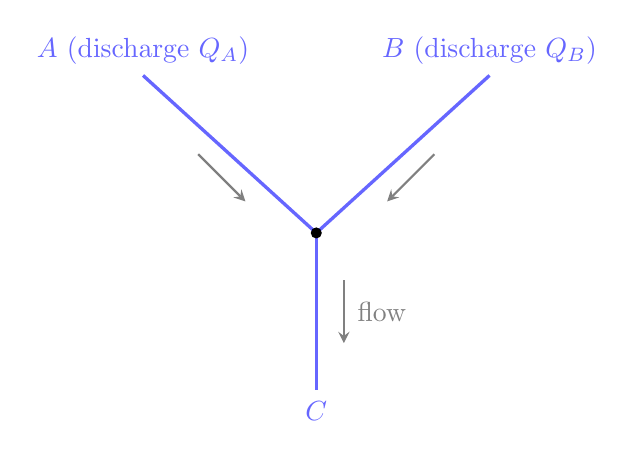
\begin{tikzpicture}[scale=1.0, >=stealth]
  \draw[very thick, blue!60] (-2.2,2) -- (0,0) node[pos=0.0, above] {$A$ (discharge $Q_A$)};
  \draw[very thick, blue!60] (2.2,2) -- (0,0) node[pos=0.0, above] {$B$ (discharge $Q_B$)};
  \draw[very thick, blue!60] (0,0) -- (0,-2) node[pos=1, below] {$C$};
  \draw[->, thick, gray] (-1.5,1.0) -- (-0.9,0.4);
  \draw[->, thick, gray] (1.5,1.0) -- (0.9,0.4);
  \draw[->, thick, gray] (0.35,-0.6) -- (0.35,-1.4);
  \node[gray, right] at (0.4,-1.0) {flow};
  \fill (0,0) circle (2pt);
\end{tikzpicture}
\caption{A confluence. Tail-down: $A$, $B$ and $C$ are correlated by distance along the river, $A$ and $B$ through the confluence. Tail-up: $C$ starts from $\{Q_A u(A^-) + Q_B u(B^-)\}/(Q_A + Q_B)$, the discharge-weighted average of the values at the downstream ends of $A$ and $B$, which are independent. Symmetric Whittle--Mat\'ern: $A$, $B$ and $C$ meet with the same weight whatever their discharge.}
\label{fig:junction}
\end{figure}

The symmetric Whittle--Mat\'ern field with Kirchhoff conditions \citep{bolin2024}, used in earlier versions of the model, ignores the direction of flow and gives every edge at a vertex the same weight, so that a seasonal stream and the Nile influence each other equally at their confluence. Its variance is $2\sigma_u^2$ at a free end of the network and smaller near confluences, an artefact of the vertex conditions: with 32{,}510 headwater ends, the variance of $u$ would be twice as large on the small streams, the main breeding habitat, as on the rivers they feed. It was therefore discarded in favour of the directed fields of \citet{bolin2026dir}.

The tail-down field runs the recursion upstream from each outlet, so that at a confluence both tributaries start from the value at the confluence. Its variance is $\sigma_u^2$ everywhere and
\[
\Cov\{u(s), u(t)\} = \sigma_u^2 \exp\{-2\,d(s, t)/r\}
\]
for points on the same river system, including points on different tributaries; different river systems are independent. This is the exponential tail-down model of \citet{verhoef2010}: suitability is similar for stretches of river close along the network, whatever the direction of flow. The tail-up field runs the recursion downstream from the sources, and at a confluence the outgoing river starts from the discharge-weighted average $\sum_k p_k u_k$ of the incoming values, with $p_k = Q_k / \sum_j Q_j$ (condition K1 of \citealp{bolin2026dir}). Then $\Cov\{u(s), u(t)\} = \Var\{u(t)\}\, e^{-2d(s,t)/r} \prod_v p_v$ when $t \rightsquigarrow s$, the product running over the confluences passed and $p_v$ being the share of discharge carried by the branch of $t$, and 0 when neither point is downstream of the other. Suitability is then a property carried by the water, mixing at confluences in proportion to discharge, and stretches not connected by flow are unrelated however close they are. The third field is the sum of independent tail-up and tail-down fields, with covariance $\phi_\uparrow C_\uparrow(s,t; r_\uparrow) + (1 - \phi_\uparrow) C_\downarrow(s,t; r)$, which contains the other two as special cases and lets the data apportion the variance.

\subsection*{Results}

The three fields were compared in an earlier round of fits, made before the move to maximum likelihood, in which the regression coefficients were integrated out under a vague Gaussian distribution while $\sigma_u$, $\sigma_Z$, $a_E$, $\gamma$ and $r$ were maximised. For the comparison below, the log-likelihood with the coefficients maximised, as defined in Section~\ref{sec:model}, was evaluated at those fits; being evaluated at estimates that maximise a slightly different criterion, these values are lower bounds of the maximised log-likelihood, by at most a few tenths of a unit judging from the maximum likelihood fits of Section~\ref{sec:covfit}, and the differences between fields are far larger than this. The range was profiled over a grid of values with the other parameters maximised, the profile interpolated by a natural cubic spline in $\log r$, and then estimated jointly with the other parameters. The tail-down profile (Figure~\ref{fig:profiles}) has a broad maximum at 1{,}357~km, with an approximate 95\% interval from 434 to 2{,}602~km, and a joint estimate of 1{,}017~km on the same plateau; the tail-up profile peaks at 520~km. At every range the tail-down field fits better; at the joint estimates its log-likelihood is $-1206.70$, against $-1231.68$ for the tail-up field, 25 units lower. In the summed field the tail-up part takes 5\% of the variance and improves the log-likelihood by 0.8 units ($-1205.93$), within the numerical error; the profile over $\phi_\uparrow$ gives an approximate interval from 0 to 0.3.

\begin{figure}[H]
\centering
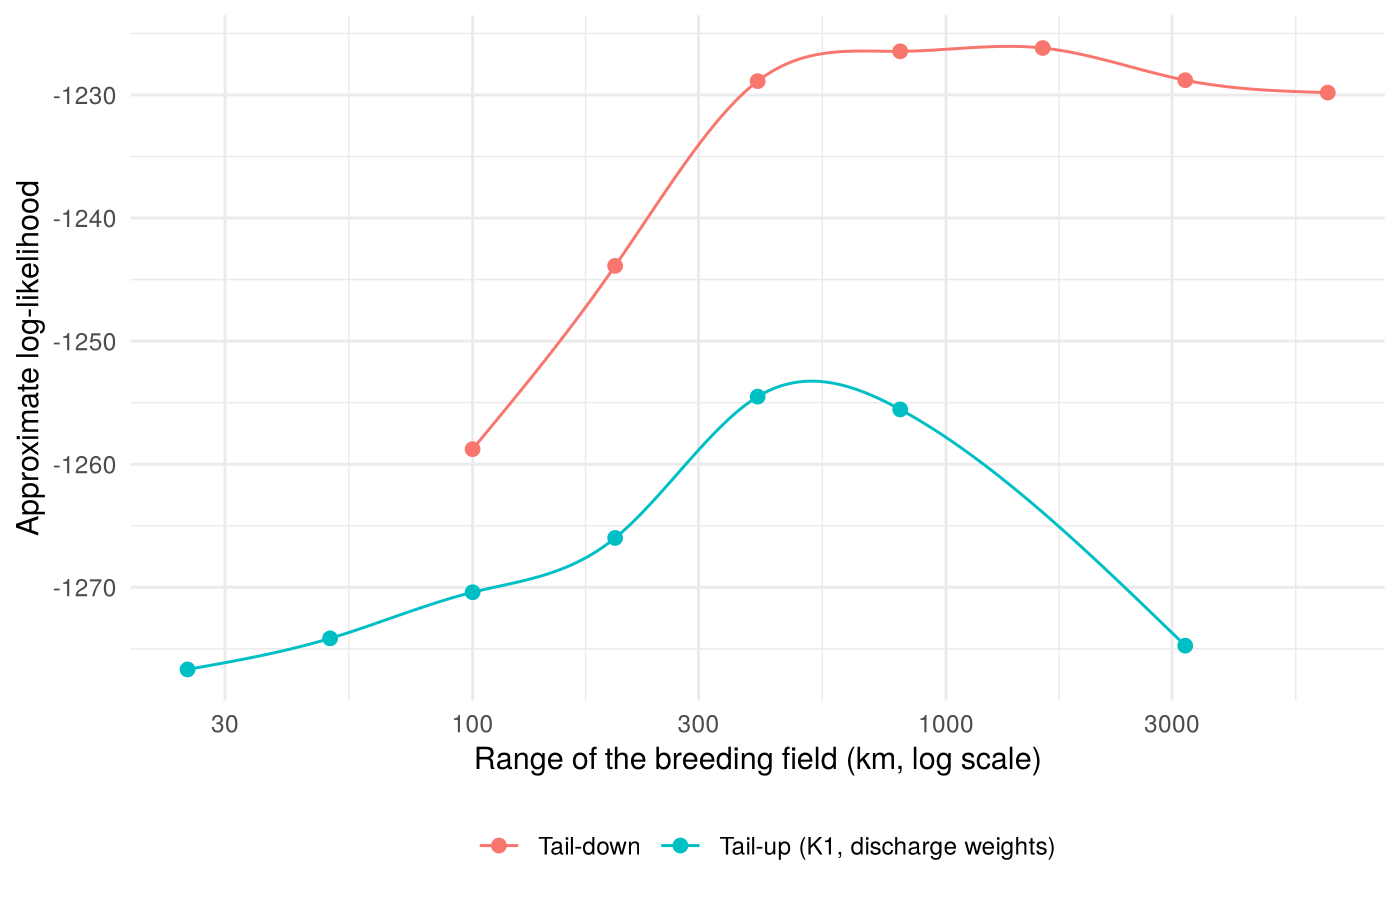
\includegraphics[width=0.66\textwidth]{directed_profiles.png}
\caption{Profile log-likelihood (earlier round of fits) over the range of the breeding field for the tail-down and tail-up fields; each point is maximised over the other parameters, and the curves are natural cubic splines in $\log r$.}
\label{fig:profiles}
\end{figure}

\begin{table}[H]
\centering
\small
\caption{Estimates from the earlier round of fits (standard errors of the regression coefficients, conditional on the other parameters, in brackets), log-likelihood with the coefficients maximised, and ten-fold cross-validation of the zero-inflated model with each breeding field. 550 villages had no positives, 14 of them in the sub-humid and humid class.}
\label{tab:fields}
\begin{tabular}{lrrr}
\toprule
 & Tail-down & Tail-up (K1) & Tail-up + tail-down \\
\midrule
Range $r$ (km) & 1017 & 514 & 967 (tail-down part) \\
Tail-up share of variance $\phi_\uparrow$ & 0 & 1 & 0.05 \\
$\sigma_u$ / $\sigma_Z$ & 7.47 / 0.50 & 5.47 / 0.45 & 7.47 / 0.50 \\
$a_1$ ($\log\AI$, $\mathrm{logit}\,\pi$) & 1.89 (0.55) & 3.62 (0.49) & 1.88 (0.54) \\
$a_E$ / $\gamma$ ($\log E$) & 0.50 / 0.10 & 0.88 / 0.19 & 0.50 / 0.10 \\
$b_1$ ($\log\AI$, $\log\lambda$) & 0.53 (0.12) & 0.95 (0.11) & 0.53 (0.12) \\
$\theta$ ($\log Q$, breeding) & $-0.48$ (0.32) & 0.24 (0.16) & $-0.53$ (0.35) \\
Log-likelihood & $-1206.70$ & $-1231.68$ & $-1205.93$ \\
\midrule
Total logarithmic score & $-1171.1$ & $-1190.8$ & $-1170.3$ \\
Area under the ROC curve / Brier score & 0.952 / 0.082 & 0.950 / 0.086 & 0.952 / 0.082 \\
Expected villages without positives (550) & 547.8 & 555.0 & 547.7 \\
\quad of which sub-humid and humid (14) & 22.4 & 30.9 & 22.9 \\
Largest deviation of the mean PIT ($p$) & 0.073 (0.012) & 0.041 (0.31) & 0.077 (0.015) \\
\bottomrule
\end{tabular}
\end{table}

The tail-up field also predicts worse (Table~\ref{tab:fields}): its total logarithmic score is about 20 units lower, discrimination is worse, and it predicts 31 villages without positives among the humid villages against 14 observed. Without a component shared by neighbouring streams, the regional contrasts that the tail-down field attributes to the rivers are taken up by aridity and by the exposure coefficients, which become larger, and the coefficient of discharge changes sign. Among villages with positives, the tail-up field is better calibrated (Figure~\ref{fig:pitfields}): the mean PIT of the tail-down field lies above the identity between about 0.4 and 0.75, by at most 0.073, meaning that where infection occurs it predicts slightly too many positives, a shift of a few percentage points rather than an error of dispersion. The variogram of the predicted village effects of the tail-down model, among the 350 villages with positives, shows no positive spatial correlation (Figure~\ref{fig:variogram}; one-sided test $p = 0.998$), so that the field accounts for the spatial structure and the village effects can be kept independent. The tail-down field (Figure~\ref{fig:umaps}) varies smoothly over whole sub-basins: high on the Nile between Abu Hamad and the Atbara confluence, across the Fourth and Fifth Cataracts, and over the small streams of the far west and south of South Sudan, and low over the Bahr el Ghazal, the White Nile and the rivers of the east.

The tail-down field was therefore selected. The suitability of the rivers for breeding appears to be shared by neighbouring streams, whether or not they are connected by flow, and to vary mainly between sub-basins, as expected if it reflects terrain, geology and climate rather than properties carried by the water. This points to measured characteristics of the rivers as covariates.

\begin{figure}[H]
\centering
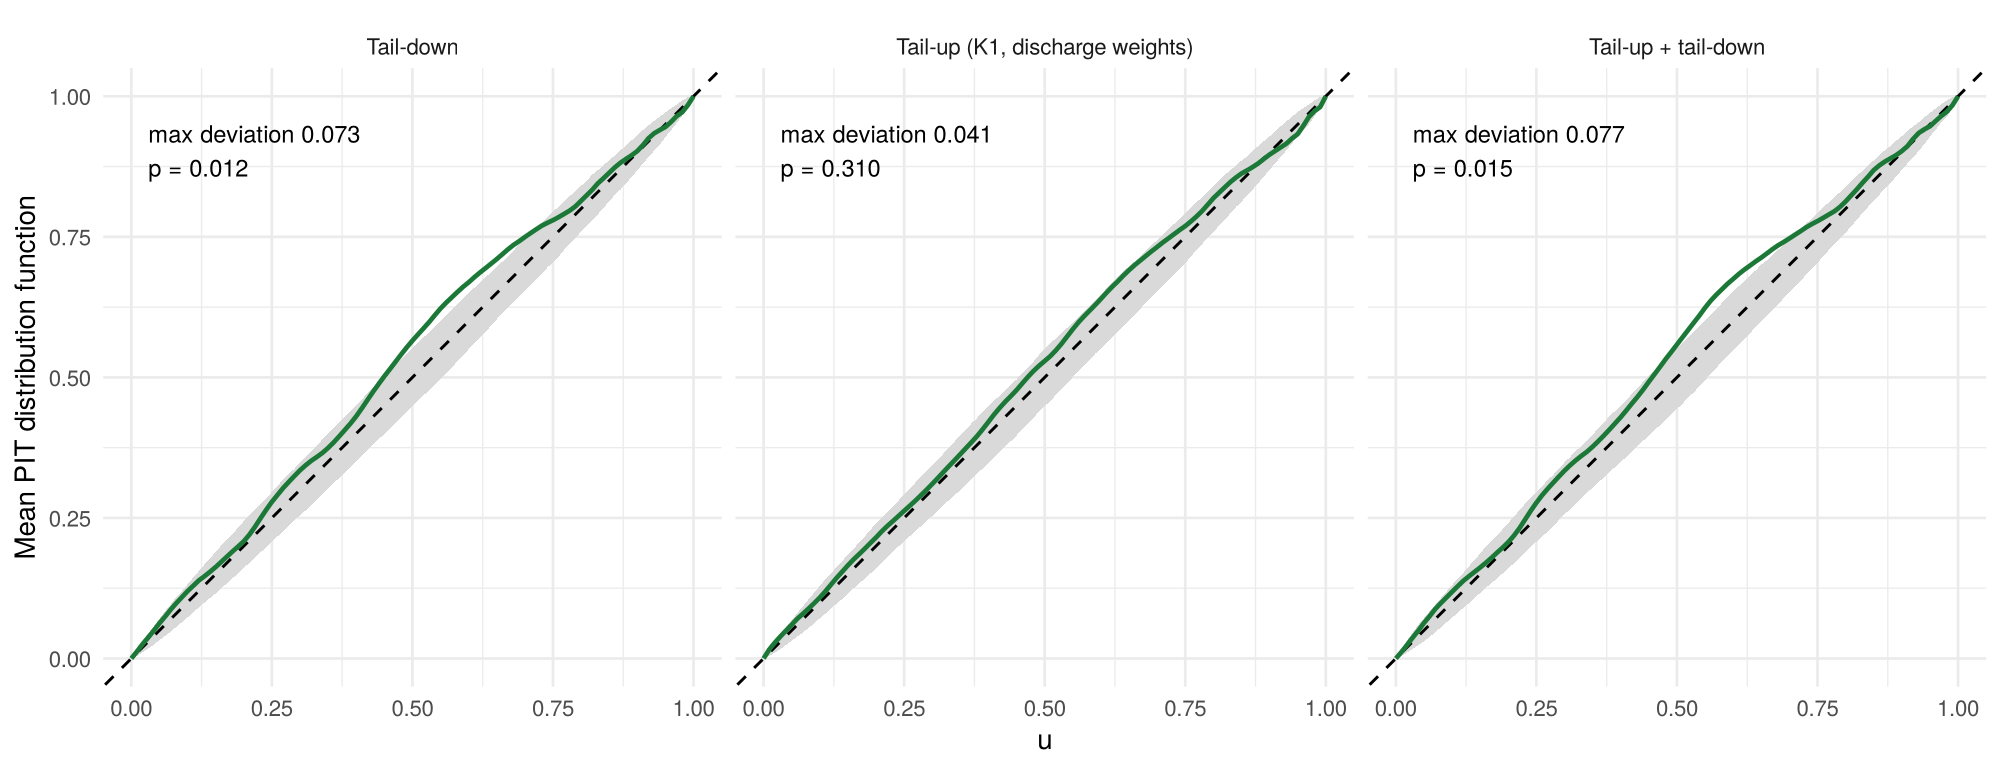
\includegraphics[width=\textwidth]{directed_pit_cdf.png}
\caption{Mean non-randomised PIT distribution function among the 350 villages with at least one positive, conditional on $Y \geq 1$, from ten-fold cross-validation. Dashed: identity; grey: pointwise 95\% band from 1{,}000 simulated sets of counts.}
\label{fig:pitfields}
\end{figure}

\begin{figure}[H]
\centering
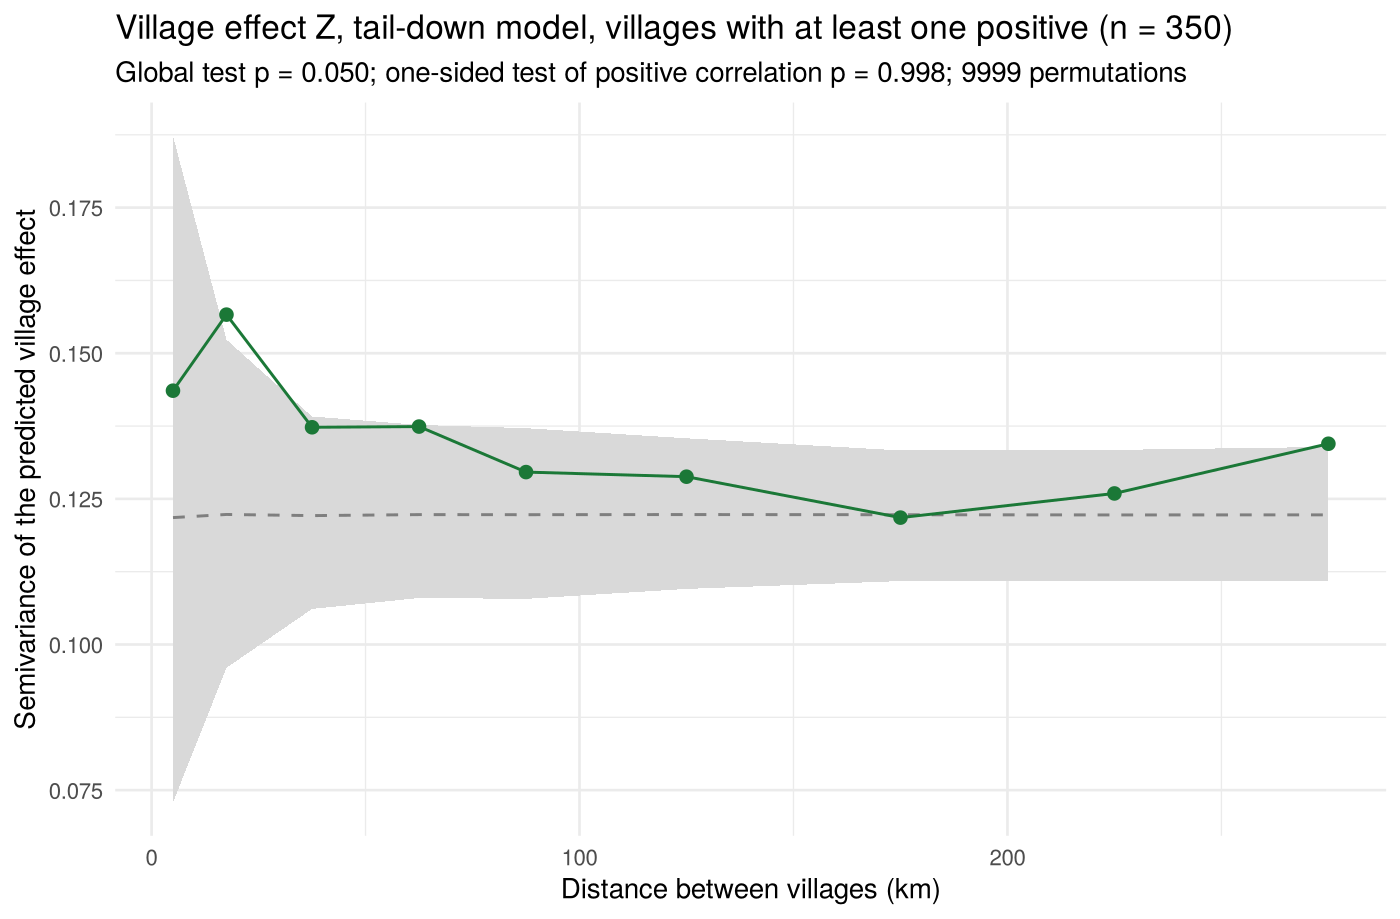
\includegraphics[width=0.6\textwidth]{variogram_z_taildown.png}
\caption{Empirical variogram of the predicted village effects in the tail-down model, villages with at least one positive, with the 95\% envelope of 9{,}999 permutations.}
\label{fig:variogram}
\end{figure}

\begin{figure}[H]
\centering
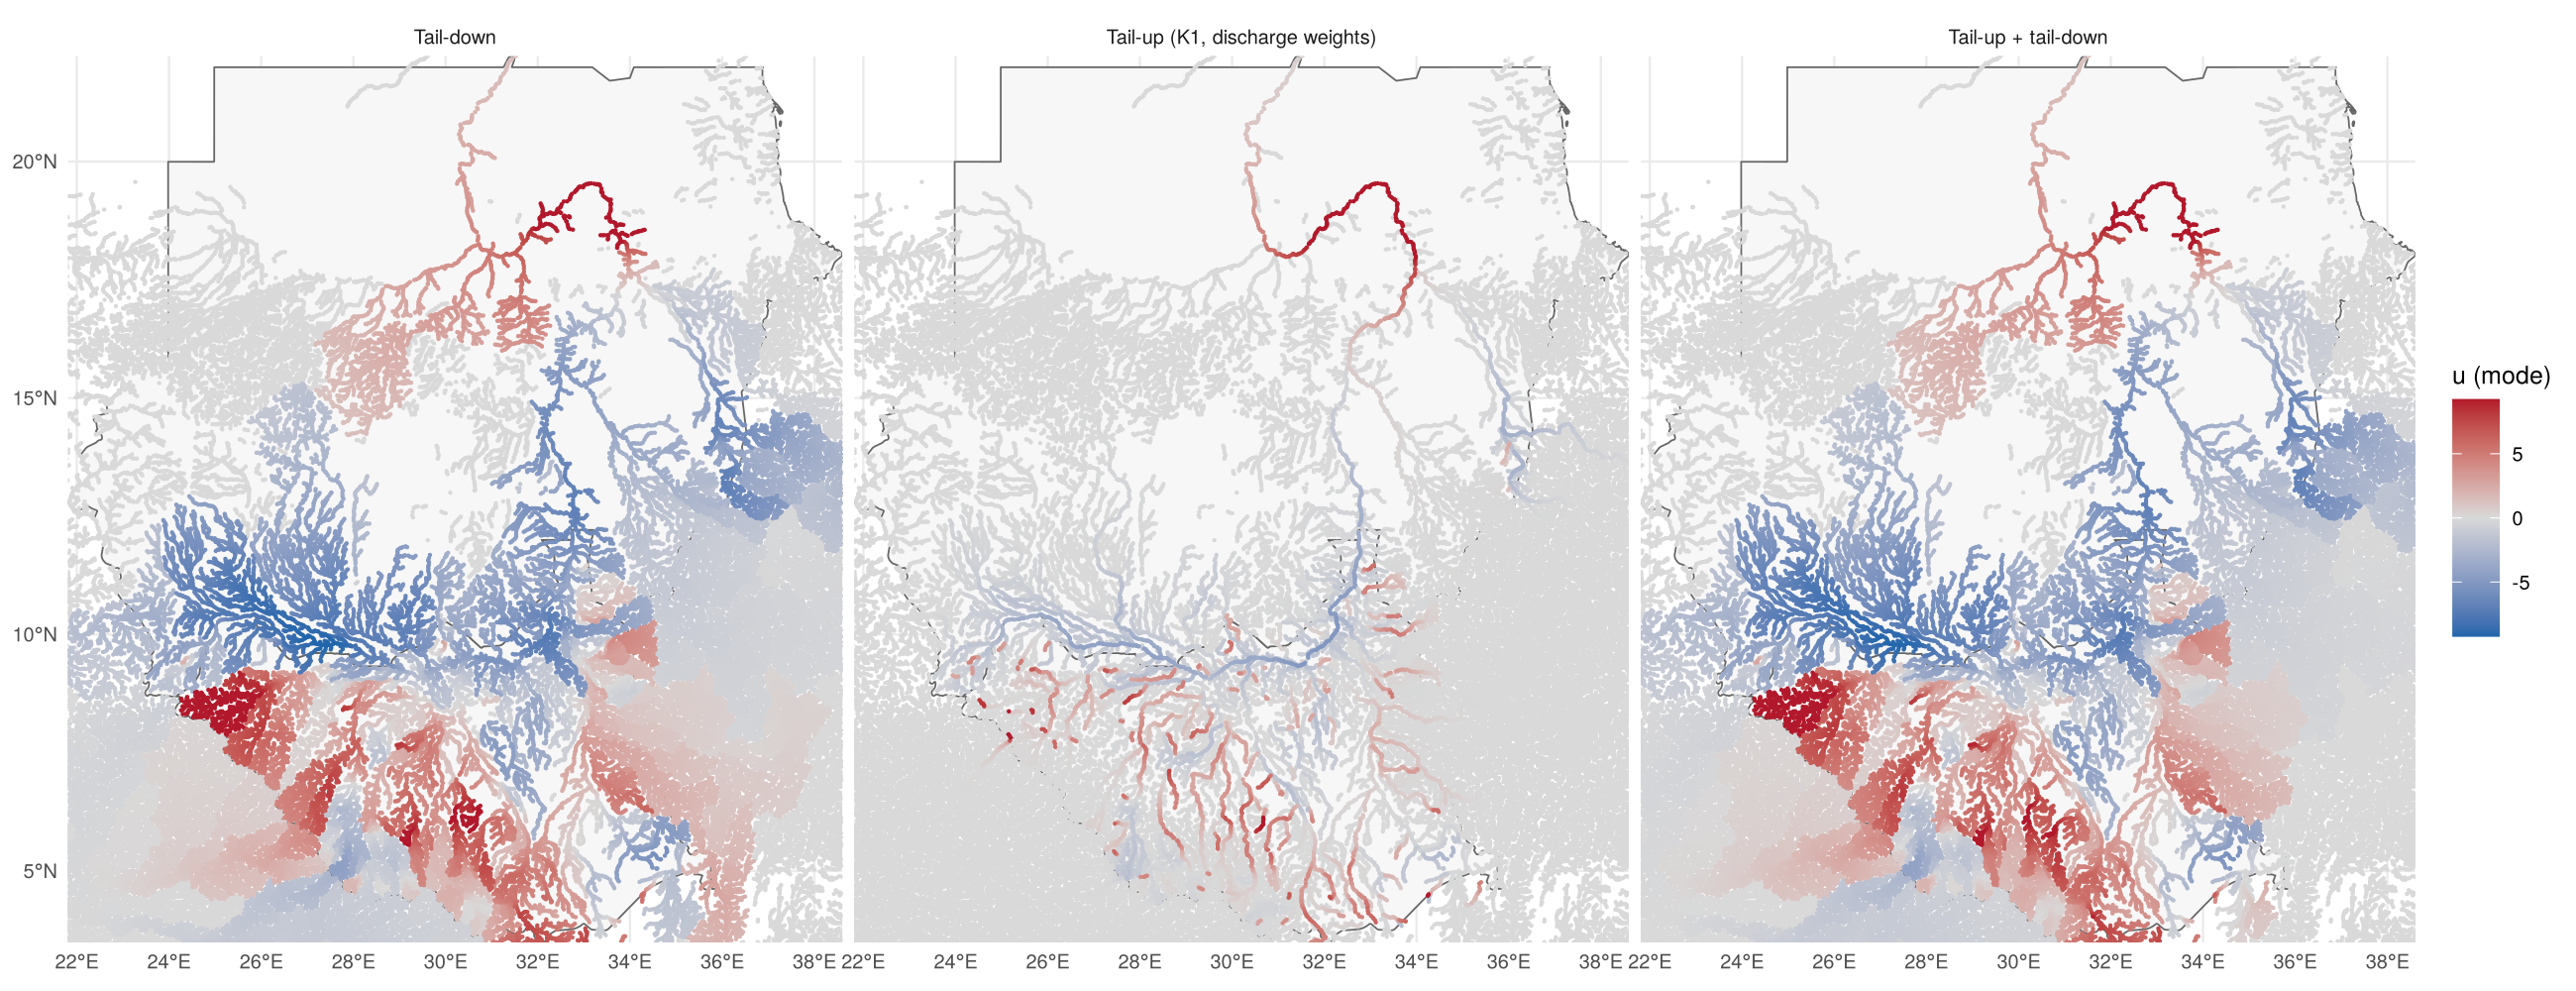
\includegraphics[width=\textwidth]{directed_joint_u_maps.png}
\caption{Posterior mode of the breeding field $u$ along the river network for the three fields.}
\label{fig:umaps}
\end{figure}

\section{Selection of habitat covariates}\label{sec:covsel}

\subsection*{Rationale}

The larvae of \textit{S.~damnosum} s.l.\ are filter feeders attached to rocks and trailing vegetation; they need fast, turbulent, well-oxygenated water, found at rapids, falls and spillways, and water that keeps flowing during their development \citep{crosskey1990}. This fixes, before looking at the data, the expected direction of each candidate covariate available in RiverATLAS. Channel slope is the closest available proxy for current speed and turbulence and should increase breeding; the velocity proxy $0.27 \log Q + 0.5 \log S$, from Manning's equation with hydraulic geometry, is a linear combination of log discharge, already in the model, and log slope, and so adds nothing beyond slope. Flow permanence, the ratio of the driest month's discharge to the mean, should increase breeding, since intermittent rivers interrupt larval development. Inundation, the extent of floodplain and swamp upstream, marks slow and silty water and should decrease breeding. These are the primary candidates. Hard rock, a reach on crystalline basement or volcanic rocks in the GLiM classification \citep{hartmann2012}, provides rapids and stable substrate; forest cover provides trailing vegetation and shade for adults, but upstream forest cover is also a proxy of regional climate. These are secondary. Lakes and dams have opposing effects (outlets and spillways are productive breeding sites, but reservoirs drown rapids), and elevation and runoff have no mechanism beyond relief, captured by slope, and rainfall, captured by aridity; these have weak rationale. Covariates of the breeding intensity should describe the larval habitat of a reach; conditions that act on adult survival, biting or people belong in the village-level parts of the model.

\subsection*{From a covariate on the river to a covariate at the village}

The covariates are defined along the rivers and the outcomes at villages, and the model indicates how to link them. With $\log w = \theta \log Q + \beta x$ for a covariate $x$, the exposure of village $i$ is $E_i(\beta) = \sum_j K_{ij} w_j$, with kernel weights $K_{ij}$ over the river nodes $j$ within 40~km, and
\[
\log E_i(\beta) = \log E_i(0) + \beta\, \bar{x}_i + O(\beta^2), \qquad
\bar{x}_i = \frac{\sum_j K_{ij} w_j(0)\, x_j}{\sum_j K_{ij} w_j(0)} .
\]
To first order a river covariate acts on prevalence through $\bar x_i$, the average of $x$ over the rivers within reach of the village weighted by the dispersal kernel, which can be computed without fitting any model ($\theta = 0$ here). Because $\log E$ enters $\mathrm{logit}\,\pi$ with coefficient $a_E$ and $\log\lambda$ with coefficient $\gamma$, a covariate acting through breeding should shift the two parts in the ratio $a_E/\gamma$, about 5 in the tail-down fit.

The associations were summarised by Spearman correlations of $\bar x_i$ with the indicator of at least one positive (the zone part) and with the empirical logit of prevalence among villages with positives (the intensity part), with 95\% intervals from a bootstrap that resamples $1^\circ \times 1^\circ$ cells, since villages close together share rivers. Because aridity is already in the model and is the dominant gradient, correlations were also computed within terciles of aridity; the dry tercile has only 11 villages with positives out of 300, so the middle (76) and humid (263) terciles carry the information. The kernel range was varied from 5 to 100~km: for nearly all covariates the correlations were almost constant, because the covariates vary smoothly in space, so that the choice of covariates does not depend on the range and the exploration cannot inform it.

A covariate was retained when it satisfied five conditions: a pre-specified mechanism and direction (primary or secondary rationale); a pooled association of the expected sign with a bootstrap interval excluding zero in at least one part; an association that survives aridity, with the expected sign and magnitude of at least 0.1 in the middle or humid tercile and no reversal in the other; robustness, the previous conditions holding for every kernel range from 20 to 80~km; and non-redundancy, only one of two candidates whose village averages are correlated beyond 0.7 being kept.

\subsection*{Results of the exploration}

\begin{table}[H]
\centering
\footnotesize\setlength{\tabcolsep}{4pt}
\caption{Spearman correlations of the village averages (kernel range 40~km) with the indicator of any positive (zone, 900 villages) and with the empirical logit of prevalence among villages with positives (intensity, 350 villages): pooled, with 95\% spatial block-bootstrap intervals, and within the middle and humid terciles of aridity.}
\label{tab:eda}
\begin{tabular}{llcccccc}
\toprule
 & & \multicolumn{3}{c}{Zone} & \multicolumn{3}{c}{Intensity} \\
\cmidrule(lr){3-5}\cmidrule(lr){6-8}
Covariate & Sign & Pooled & Middle & Humid & Pooled & Middle & Humid \\
\midrule
log discharge & ref. & $-0.45$ ($-0.54$, $-0.34$) & $-0.30$ & 0.12 & $-0.06$ ($-0.21$, 0.07) & $-0.13$ & 0.10 \\
log slope & $+$ & 0.37 (0.21, 0.50) & 0.04 & 0.16 & 0.31 (0.14, 0.46) & 0.28 & 0.10 \\
steep share & $+$ & 0.36 (0.20, 0.50) & 0.08 & 0.14 & 0.28 (0.12, 0.43) & 0.19 & 0.08 \\
velocity proxy & $+$ & $-0.02$ ($-0.20$, 0.14) & $-0.14$ & 0.23 & 0.26 (0.08, 0.41) & 0.17 & 0.22 \\
flow permanence & $+$ & 0.40 (0.23, 0.54) & $-0.10$ & $-0.11$ & 0.14 ($-0.05$, 0.29) & $-0.33$ & 0.06 \\
inundation & $-$ & $-0.52$ ($-0.63$, $-0.39$) & $-0.07$ & $-0.16$ & $-0.40$ ($-0.54$, $-0.24$) & $-0.21$ & $-0.18$ \\
hard rock & $+$ & 0.40 (0.23, 0.54) & 0.04 & 0.22 & 0.39 (0.23, 0.52) & 0.25 & 0.21 \\
forest & $+$ & 0.45 (0.31, 0.58) & 0.01 & 0.22 & 0.42 (0.26, 0.55) & 0.06 & 0.31 \\
lakes & ? & $-0.39$ ($-0.51$, $-0.24$) & $-0.06$ & $-0.01$ & $-0.22$ ($-0.40$, $-0.03$) & $-0.14$ & $-0.03$ \\
regulation & ? & $-0.46$ ($-0.57$, $-0.34$) & $-0.10$ & $-0.03$ & $-0.28$ ($-0.39$, $-0.17$) & $-0.17$ & $-0.09$ \\
elevation & none & 0.50 (0.36, 0.62) & 0.08 & 0.12 & 0.33 (0.14, 0.50) & 0.19 & 0.09 \\
runoff & none & 0.51 (0.36, 0.63) & 0.18 & 0.21 & 0.20 (0.06, 0.34) & $-0.14$ & 0.12 \\
\bottomrule
\end{tabular}
\end{table}

Every covariate is associated with risk in the pooled data (Table~\ref{tab:eda}), including elevation and runoff, which have no mechanism of their own: the humid south-west has steep rivers on basement rock, forest, little floodplain and most of the transmission. Within aridity terciles the correlations fall to 0.1--0.3, and there the covariates separate. Figures~\ref{fig:partzone} and \ref{fig:partint} show the village averages against the two parts of the model, with binomial and quasi-binomial smooths, and Figure~\ref{fig:uvscov} the posterior mode of $u$ in the tail-down model without covariates against the covariates at the river nodes within 40~km of a village, which shows what part of the breeding field each covariate could explain and in what functional form.

Channel slope satisfies all five conditions. The share of villages with positives rises from about 25\% in the lower quintiles of the village average to 80\% in the highest, prevalence among villages with positives rises from 11\% to 25\%, and the association persists within aridity terciles (0.16 for the zone in the humid tercile, 0.26--0.35 for intensity in the middle tercile from 30~km upwards). Its slopes on the two parts, 0.95 on the logit of any positive and 0.22 on the complementary log-log of prevalence among positive villages per standard deviation, are in the ratio 4.4 expected of a term acting through $E$. At the river nodes, $u$ is flat for slopes up to about 2~dm/km and then increases steadily with $\log(1 + \text{slope})$, by about 5 units over the observed range, so that slope enters linearly in $\log(1 + \text{slope})$. The share of steep river (slope at least 2~m/km) is correlated 0.89 with log slope and was dropped as redundant.

Inundation satisfies all conditions with the expected negative sign, consistently within terciles and across ranges, with a ratio of slopes on the two parts of 3.3. At the nodes, $u$ falls from about 0.3 where there is no inundation upstream to about $-3.6$ at $\log(1 + \text{inundation}) \approx 1.5$, about 3.5\% of the upstream area, and is roughly constant beyond, so that inundation enters as $\min\{\log(1 + \text{inundation}), 1.5\}$, a linear term with a plateau. Its village averages are correlated $-0.63$ with those of slope: the two describe the contrast between steep and flat rivers, measured independently from elevation and from satellite water mapping.

Hard rock satisfies all conditions (0.20--0.25 in the humid tercile at every range), with a ratio of 3.0. It is a class of each reach and enters as an indicator; the mean of $u$ is $-2.9$ on sediments and $1.0$ on basement or volcanic rock. It is correlated 0.66 with slope, and the lithological map is coarse, so that it carries little beyond slope; in a preliminary fit, made before the move to maximum likelihood, its coefficient added to slope and inundation was $-0.64$ (95\% interval $-3.75$ to 2.48). It is not in the final model.

Forest cover satisfies the formal conditions only through the humid tercile, and three features suggest that it marks the forested south-west rather than habitat: it is the one candidate whose association grows steadily with the kernel range (pooled from 0.32 at 5~km to 0.58 at 100~km for the zone, and from $-0.10$ to 0.21 in the middle tercile), whereas a habitat effect should be strongest for the nearest rivers; its ratio of slopes on the two parts, 8.2, is that of the climate proxies (elevation 8.9, runoff 7.2) rather than of the habitat covariates; and it measures forest over the whole upstream catchment rather than the riverside vegetation used by larvae. It was not included. Flow permanence has a strong pooled association but reverses within aridity terciles at every range, following rainfall rather than habitat. The velocity proxy changes sign with the kernel range and between the two parts, and with $\log Q$ in the model is equivalent to slope. Lakes and regulation have no fixed expected direction and no association within terciles, and elevation and runoff have no mechanism of their own; runoff is the one excluded covariate with a consistent association of about 0.2 within terciles for the zone, and could be reconsidered as a measure of the permanence of small streams.

Discharge, the only river attribute in the model of Section~\ref{sec:fields}, was examined for its functional form and for whether it is still needed with the habitat covariates. At the river nodes, $u$ is flat in $\log Q$ from 0.1 to about 55~m$^3$/s, so that the total log breeding intensity $\theta\log Q + u$ declines roughly linearly with $\log Q$; above 55~m$^3$/s, $u$ is lower, except on the largest reaches of the Nile, where it is very high: these are the cataracts of the Abu Hamad focus, where breeding on the Nile rapids is a slope effect rather than a discharge effect. Downstream, channels become flatter and floodplains wider, so that the decline of breeding with discharge is in large part the effect of slope and inundation. In a maximum likelihood fit with $\theta\log Q$ added to slope and inundation, the log-likelihood at the best point reached was within 0.1 of that of the model without it, so discharge was dropped.

\subsection*{Selected model}

The breeding intensity of the final model is
\[
\log w(s) = \beta_S \log\{1 + S(s)\} + \beta_I \min[\log\{1 + I(s)\}, 1.5] + u(s),
\]
with $S$ the channel slope of the reach (dm/km) and $I$ the long-term maximum inundation of its upstream catchment (\%), both from RiverATLAS \citep{linke2019}, and $u$ the tail-down field. The expected signs are $\beta_S > 0$ and $\beta_I < 0$.

\begin{figure}[H]
\centering
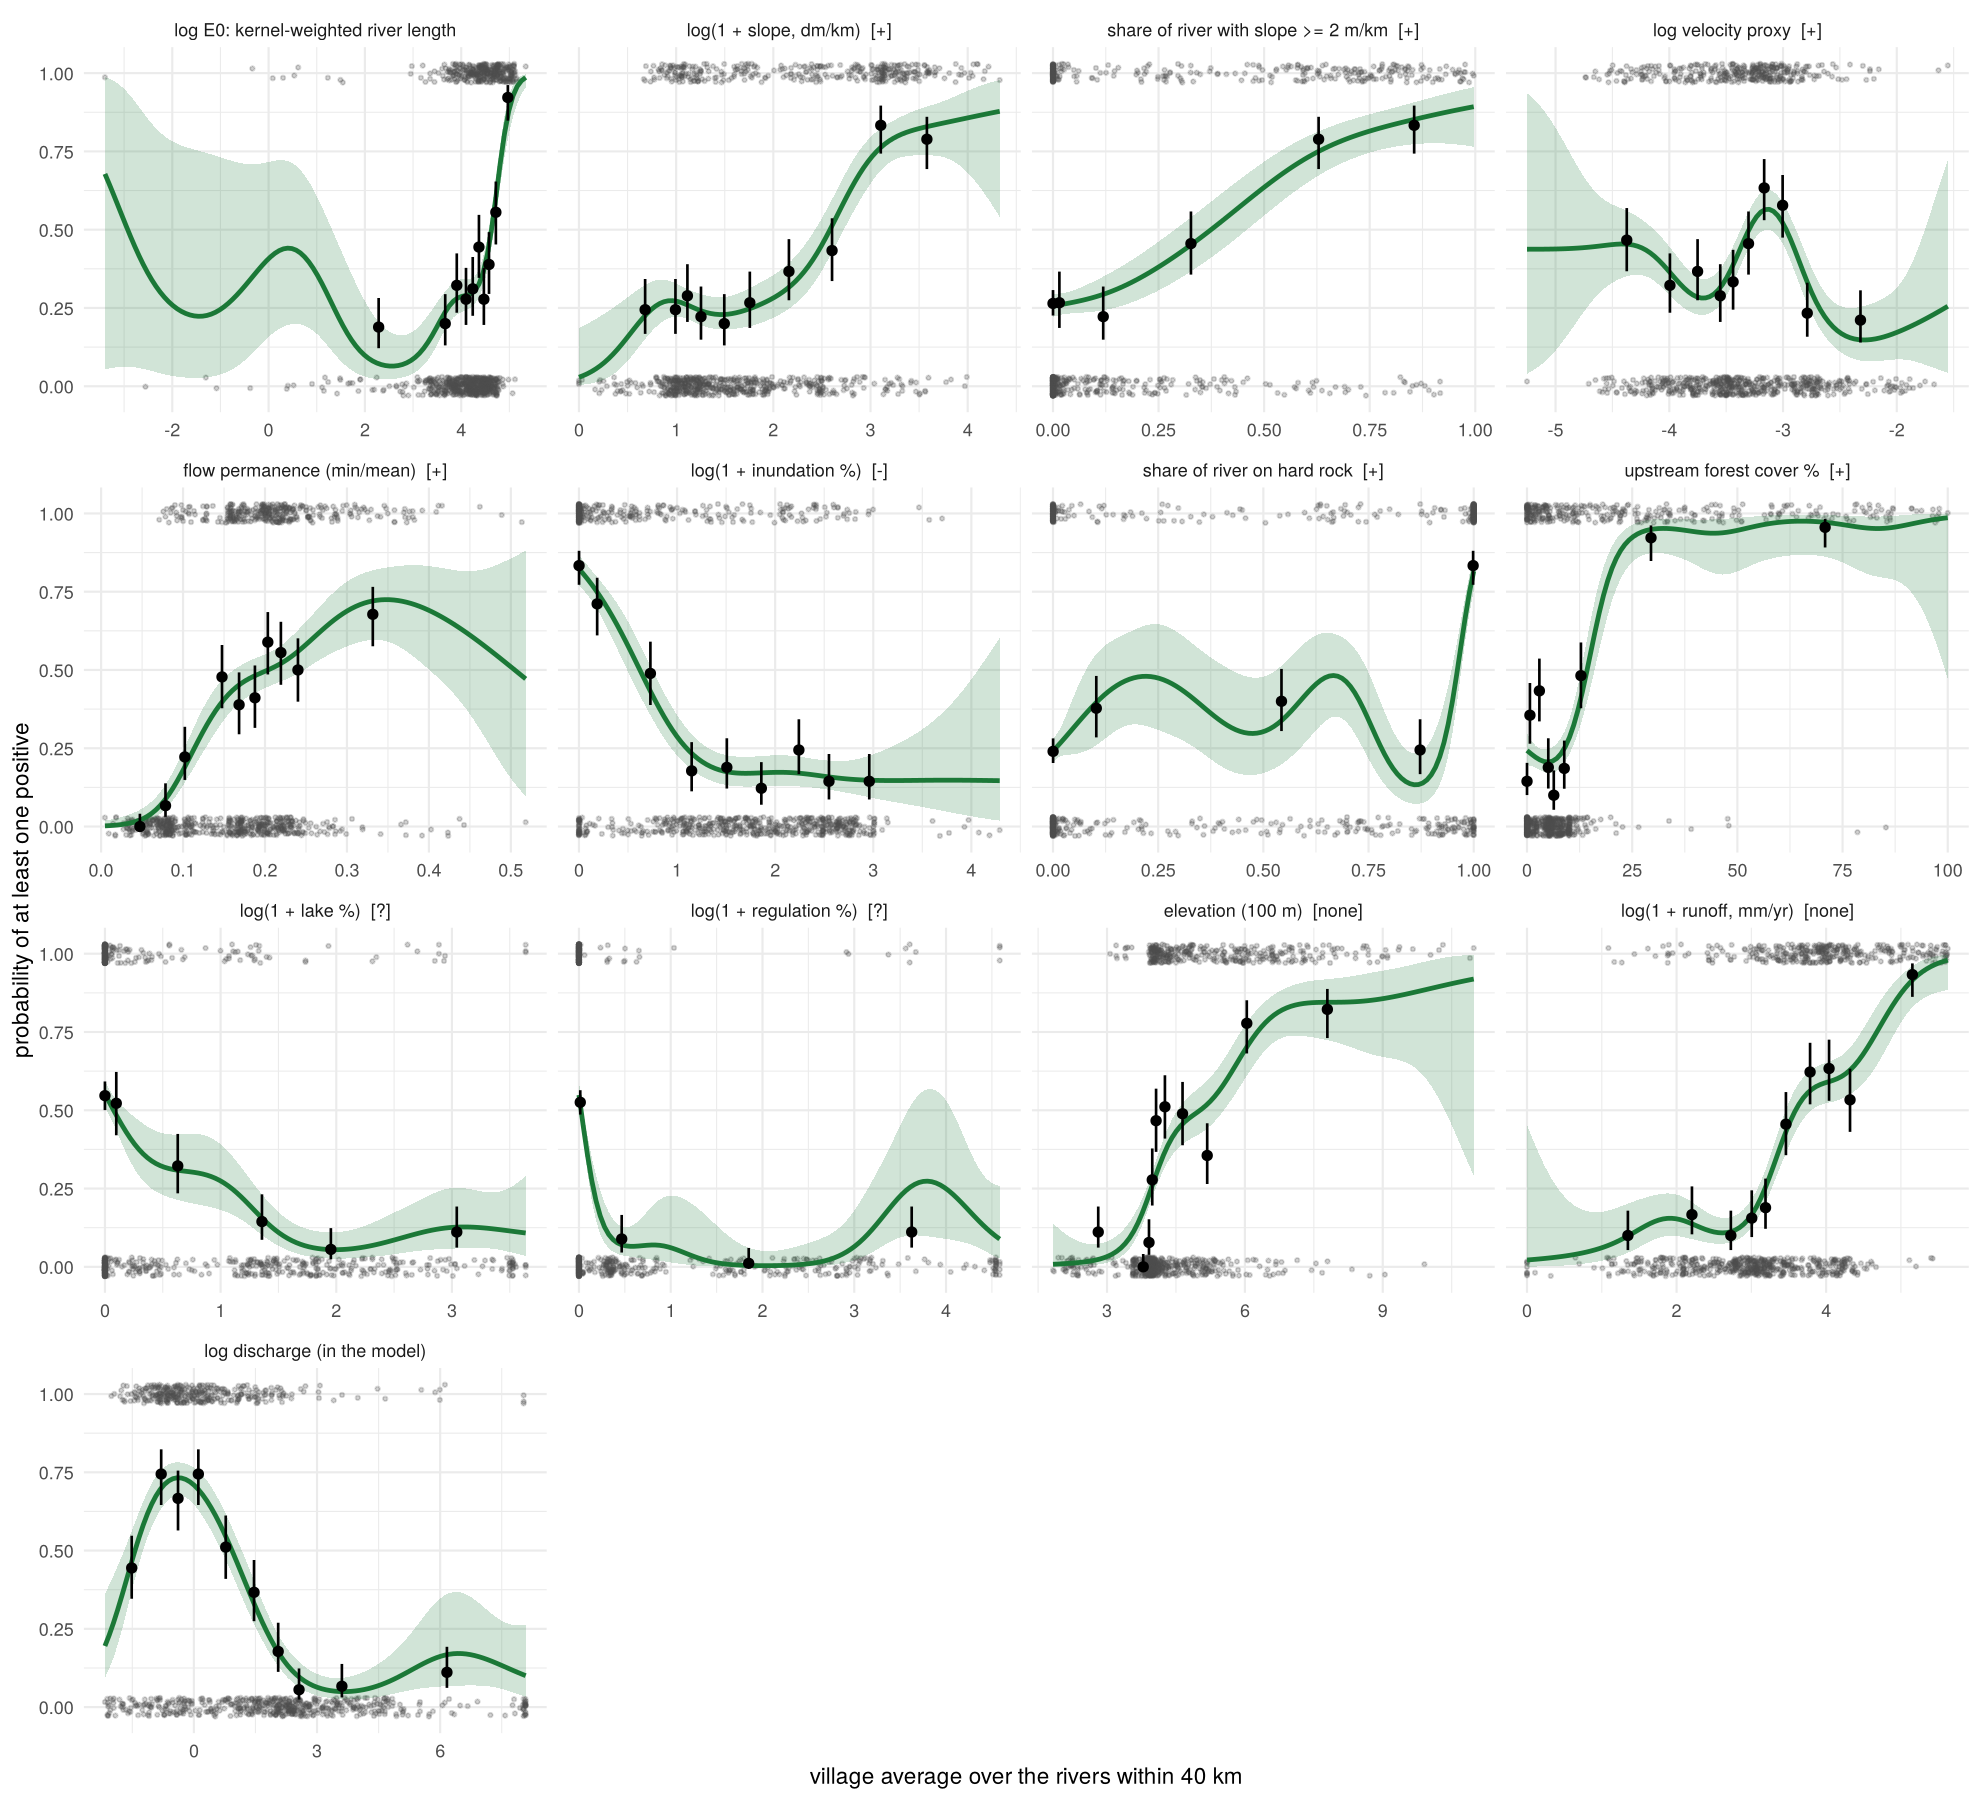
\includegraphics[width=\textwidth]{cov_part_zone.png}
\caption{Probability of at least one positive against the village average of each covariate within 40~km: villages (jittered at 0 and 1), proportions in deciles with 95\% Wilson intervals, and binomial GAM smooth with 95\% band. The first panel is $\log E_0$, the log kernel-weighted river length.}
\label{fig:partzone}
\end{figure}

\begin{figure}[H]
\centering
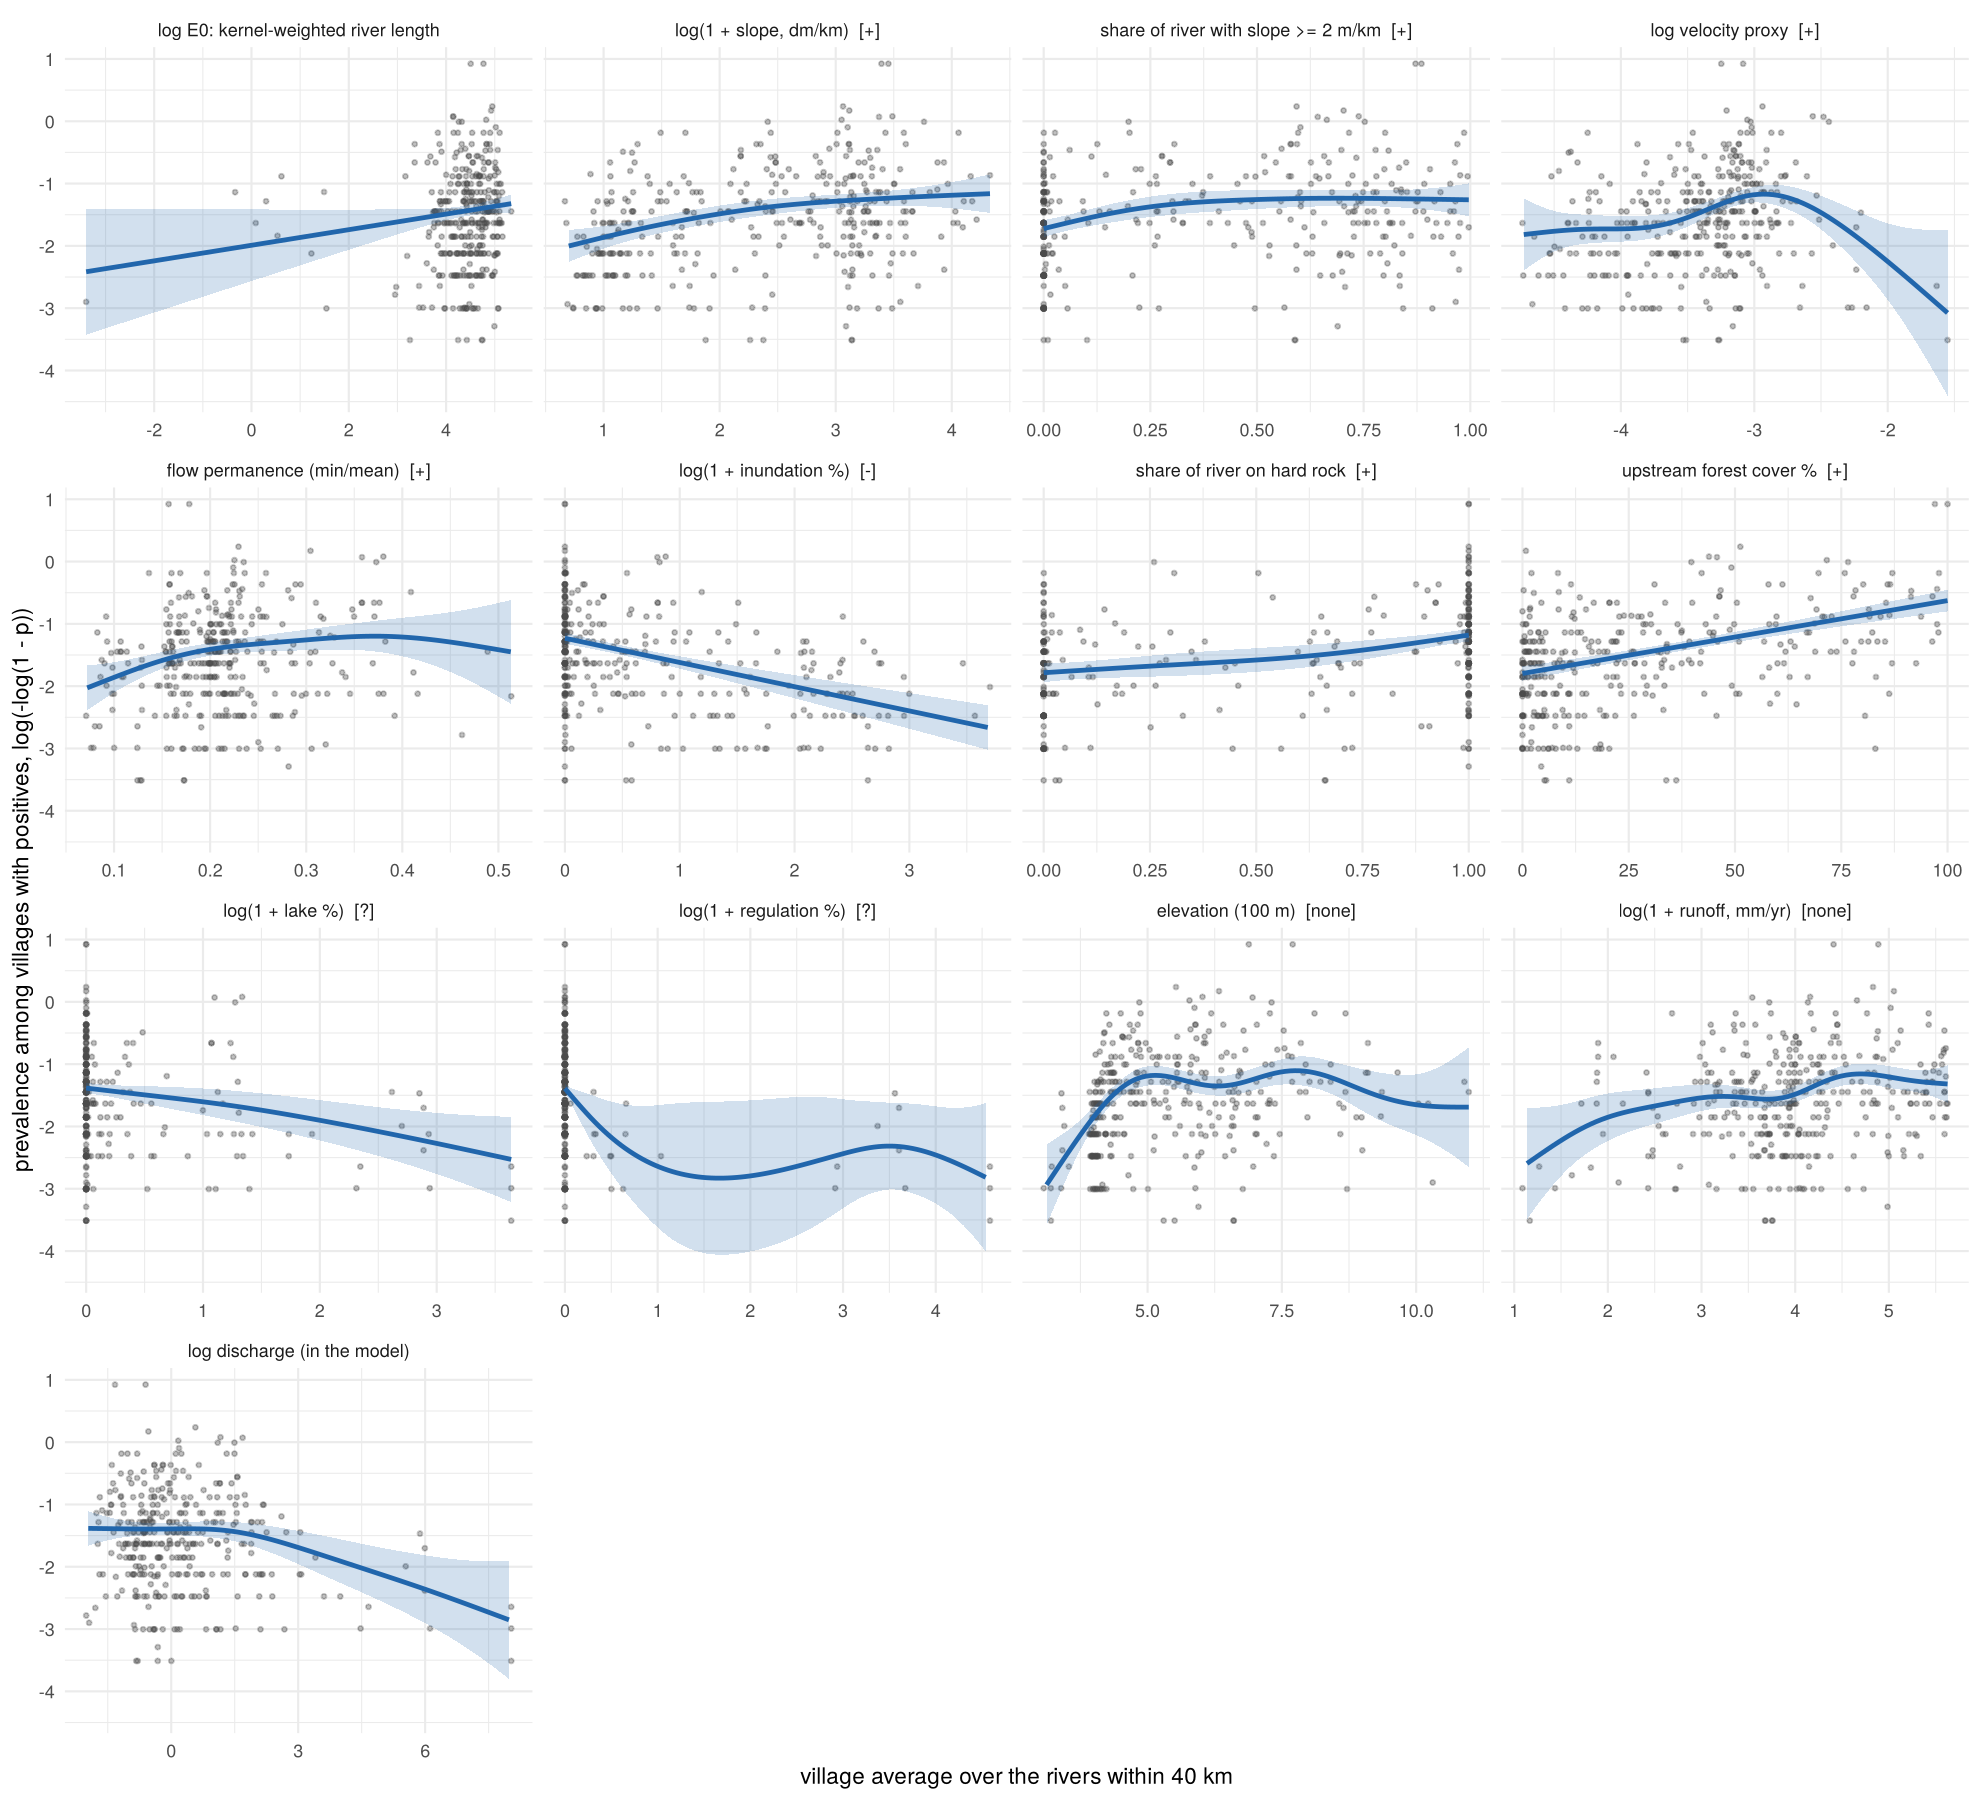
\includegraphics[width=\textwidth]{cov_part_intensity.png}
\caption{Prevalence among the 350 villages with positives, on the complementary log-log scale of $\log\lambda$, against the village average of each covariate within 40~km, with quasi-binomial GAM smooth and 95\% band.}
\label{fig:partint}
\end{figure}

\begin{figure}[H]
\centering
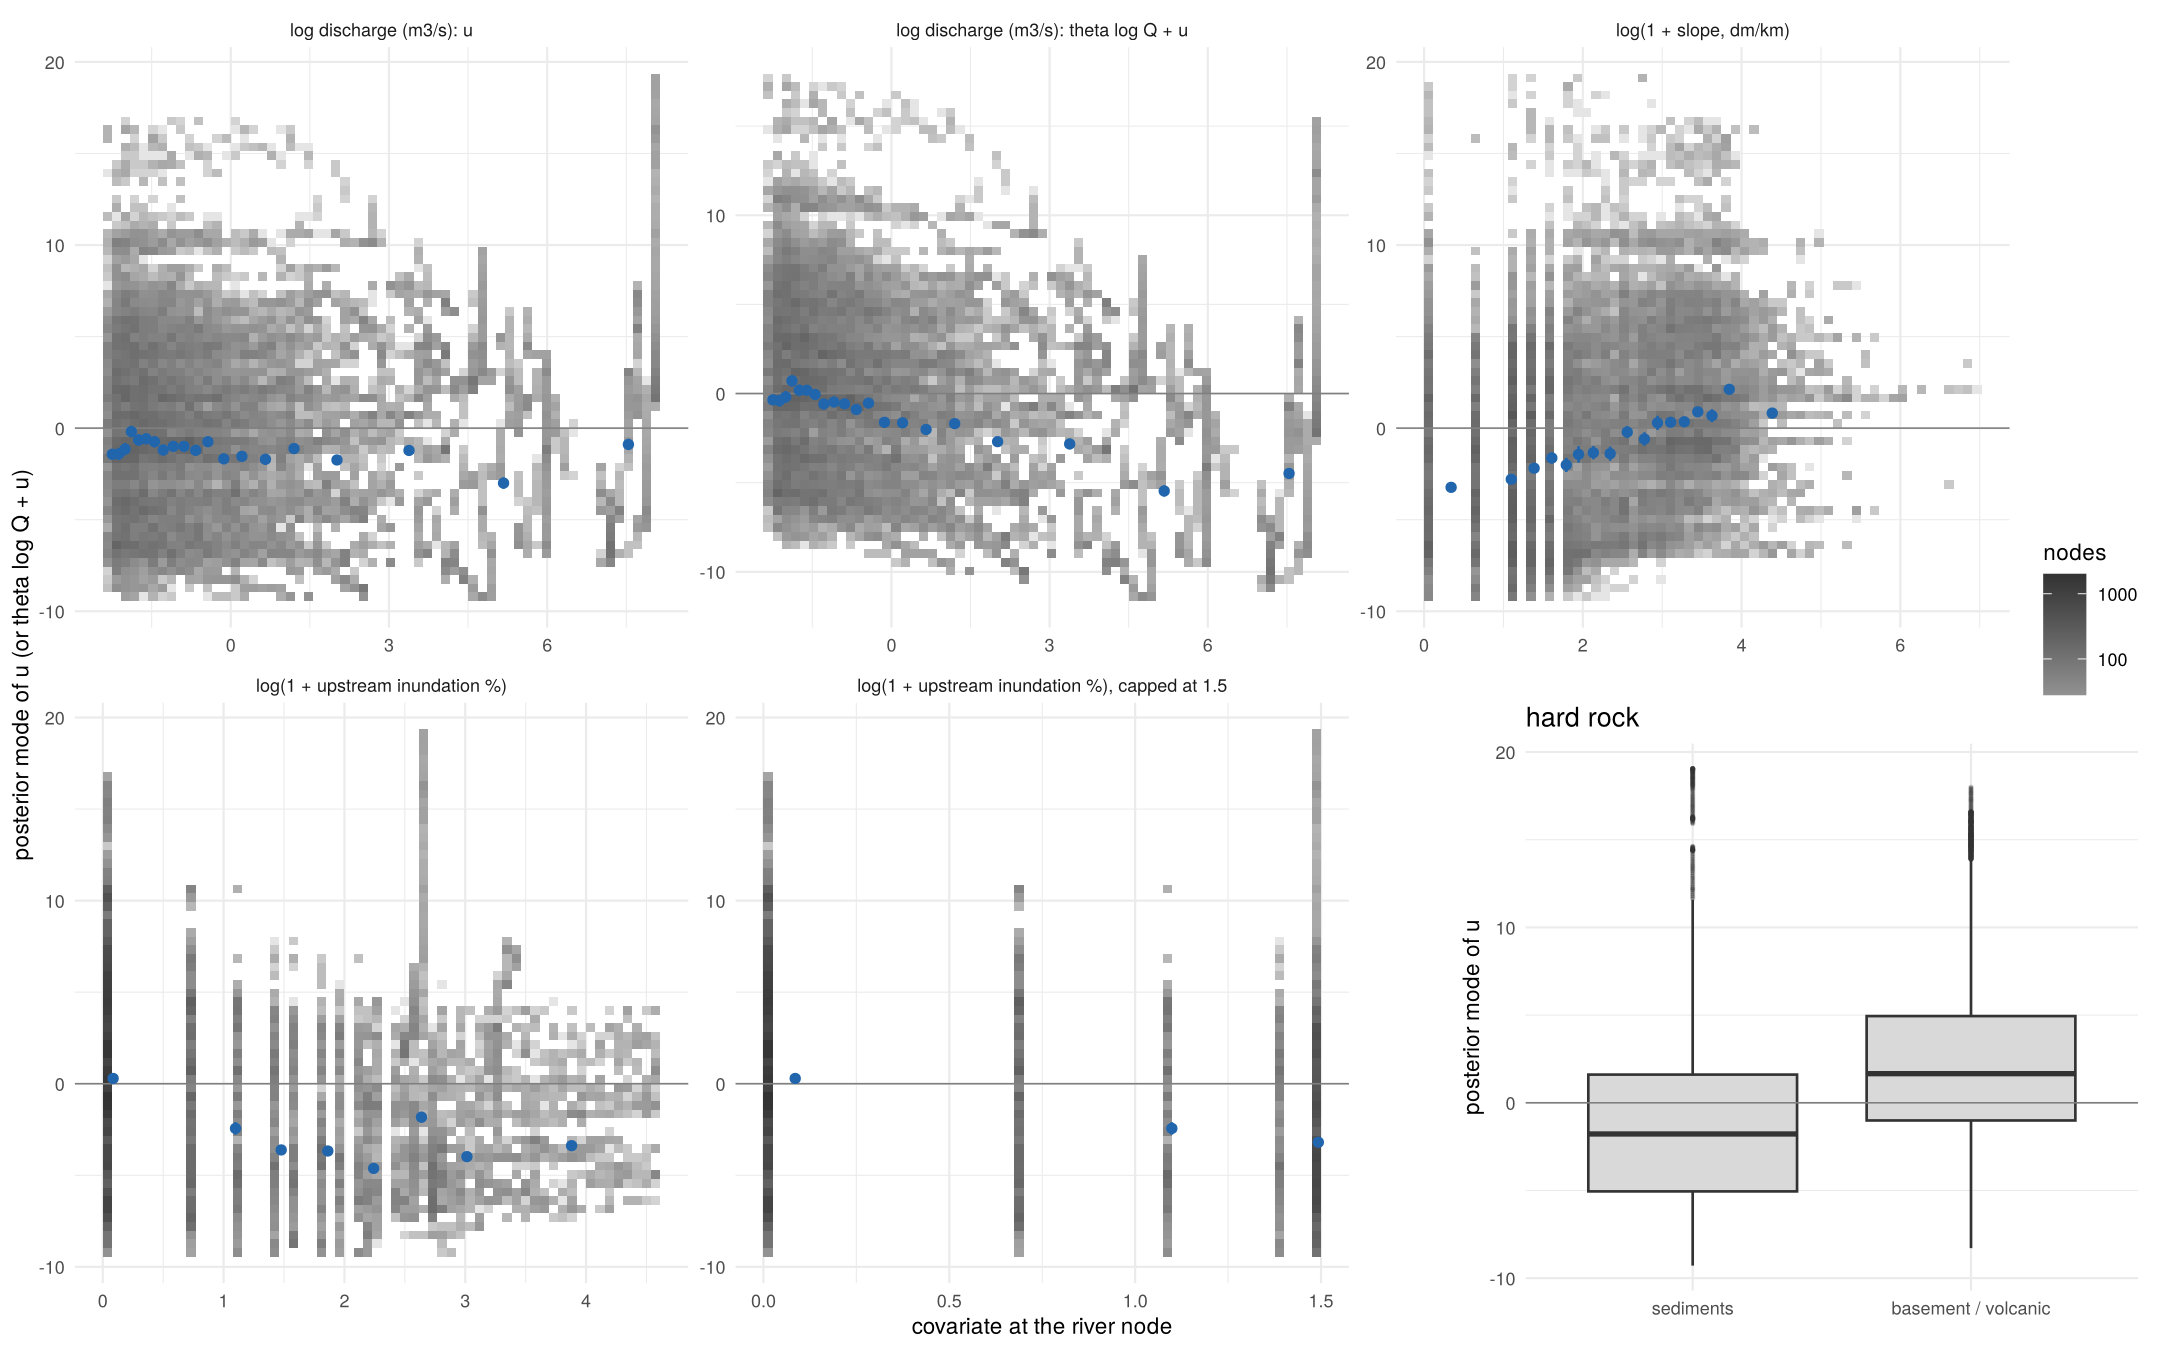
\includegraphics[width=\textwidth]{u_vs_covariates.png}
\caption{Posterior mode of the breeding field $u$ of the tail-down model without habitat covariates against discharge and the selected covariates at the 54{,}718 river nodes within 40~km of a village. Grey: number of nodes; blue: means of $u$ in bins of the covariate, weighted by the kernel weight of each node summed over villages, with 95\% intervals. The second panel shows the total log breeding intensity $\theta \log Q + u$. Hard rock: box plots of $u$ by class.}
\label{fig:uvscov}
\end{figure}

\section{Model fit with covariates}\label{sec:covfit}

The final model, M3, has the tail-down field of Section~\ref{sec:fields} and channel slope and inundation in the breeding intensity (Section~\ref{sec:covsel}). It was fitted by maximum likelihood, with no prior on any parameter. The log-likelihood has a long, flat and slightly curved ridge along which the intercept of $\mathrm{logit}\,\pi$, the two breeding coefficients, $a_E$ and $\sigma_u$ trade off, since the covariates act only through $\log E$; finite differences with equal steps in every parameter gave a wrong Hessian there. The maximisation was therefore completed by quasi-Newton (BFGS) steps in coordinates whitened by a finite-difference Hessian, and stopped when the predicted gain was below 0.01 (the last steps gained 0.005 each). The observed information was computed at the estimate by central differences along its eigenvectors, with steps of half a standard error and every inner fit started from the mode of $(u, Z)$ at the estimate; it is positive definite, and a Newton step from the estimate predicts a gain of 0.03.

\begin{table}[H]
\centering
\small
\caption{Maximum likelihood estimates of M3 with 95\% Wald intervals from the observed information. Intervals for $\sigma_u$, $\sigma_Z$ and $r$ are computed on the log scale.}
\label{tab:m3est}
\begin{tabular}{llc}
\toprule
 & Parameter & Estimate (95\% interval) \\
\midrule
Force of infection, $\log\lambda$ & $b_0$ (intercept) & $-2.01$ ($-2.51$, $-1.52$) \\
 & $b_1$ ($\log\AI$) & 0.54 (0.24, 0.83) \\
 & $\gamma$ ($\log E$) & 0.069 (0.043, 0.096) \\
Zone of transmission, $\mathrm{logit}\,\pi$ & $a_0$ (intercept) & 0.49 ($-2.34$, 3.32) \\
 & $a_1$ ($\log\AI$) & 2.17 (0.79, 3.54) \\
 & $a_E$ ($\log E$) & 0.37 (0.23, 0.51) \\
Breeding intensity, $\log w$ & $\beta_S$ ($\log(1 + \text{slope})$) & 1.83 (0.63, 3.04) \\
 & $\beta_I$ ($\min\{\log(1 + \text{inundation}), 1.5\}$) & $-2.30$ ($-3.97$, $-0.63$) \\
Breeding field $u$ & $\sigma_u$ & 9.44 (6.31, 14.11) \\
 & range $r$ (km) & 898 (409, 1969) \\
Village effects & $\sigma_Z$ & 0.49 (0.42, 0.56) \\
\midrule
 & Log-likelihood & $-1192.31$ \\
\bottomrule
\end{tabular}
\end{table}

Both habitat covariates have the expected sign, with 95\% intervals that exclude zero (Table~\ref{tab:m3est}). Breeding increases with channel slope: doubling $1 + S$ multiplies the breeding intensity by $2^{\hat\beta_S} \approx 3.6$. It decreases with inundation upstream: from no inundation to the plateau at $\log(1 + I) = 1.5$ (about 3.5\% of the catchment) it is multiplied by $\exp(-1.5\,|\hat\beta_I|) \approx 0.03$. Figure~\ref{fig:multiplier} maps the combined multiplier $\exp(\hat\beta_S h_S + \hat\beta_I h_I)$ along the rivers: it is high on the steep streams of the Ethiopian highlands, the uplands of northern Darfur and the Nile--Congo divide in the south-west, and low over the Sudd, the Bahr el Ghazal and the main Nile. Aridity remains strongly associated with both parts of the model. The breeding field keeps a large standard deviation and a range of several hundred kilometres: the covariates describe local habitat, and the field the regional variation that they do not explain.

\begin{figure}[H]
\centering
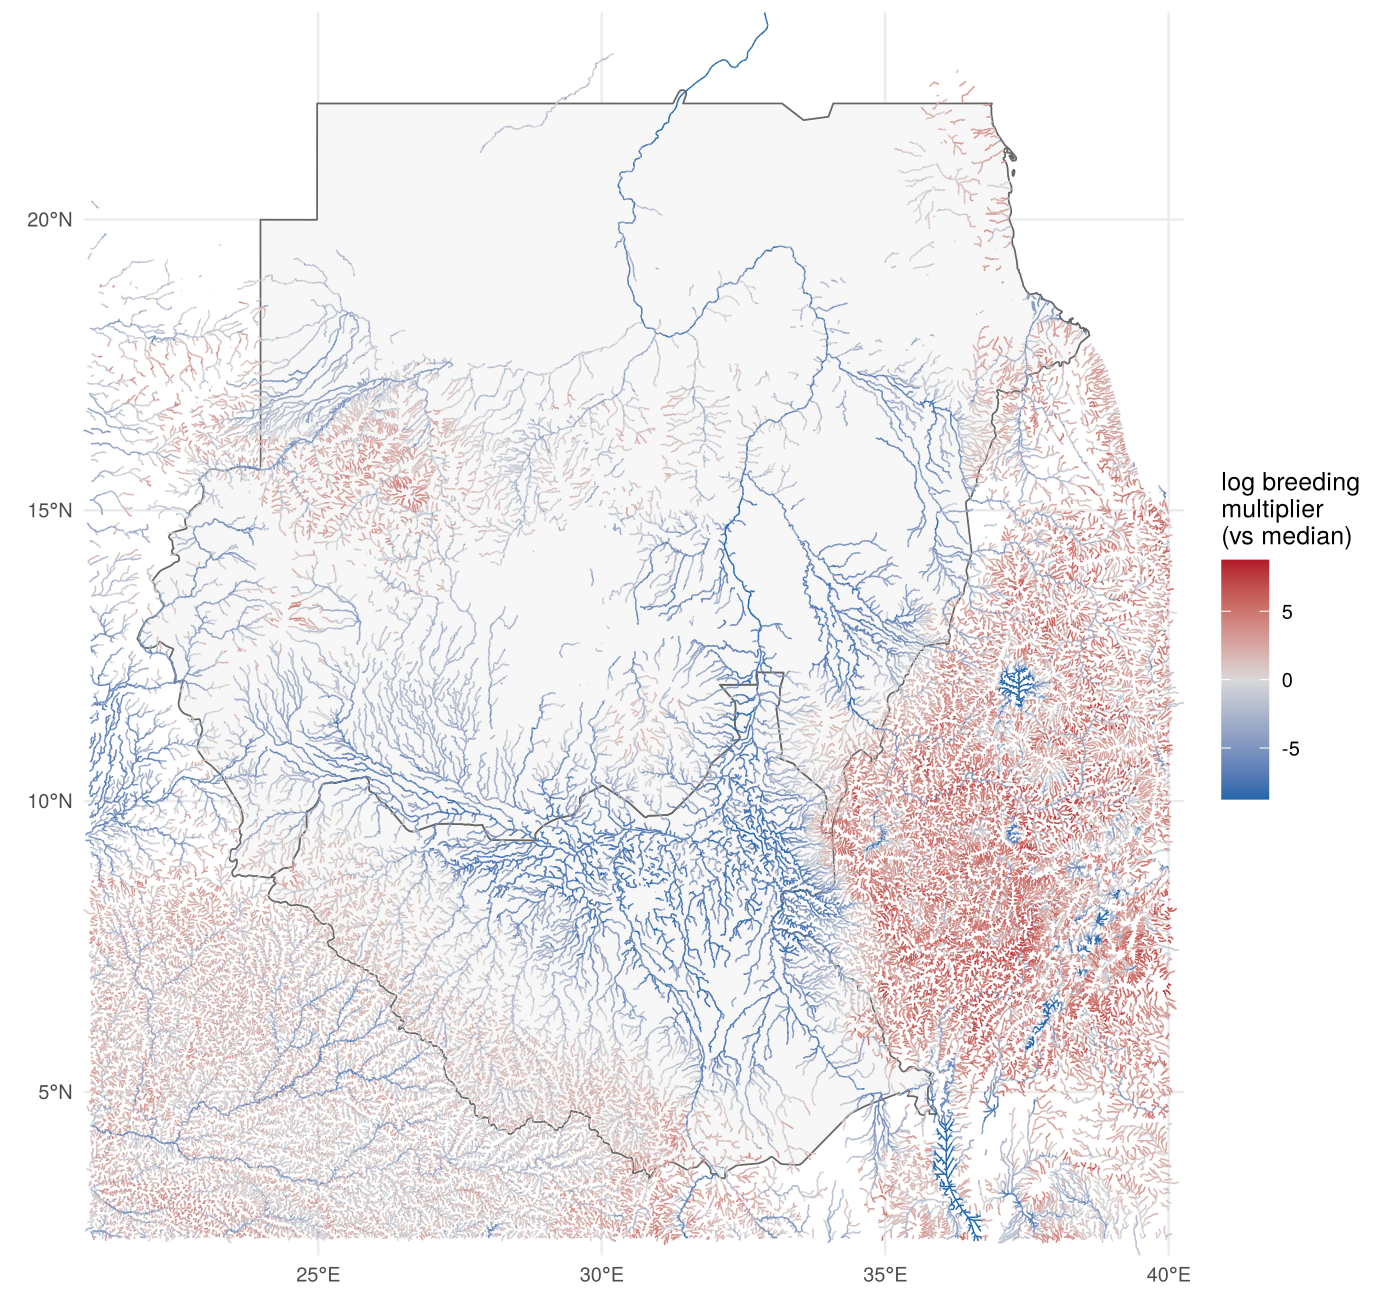
\includegraphics[width=0.62\textwidth]{cov_fit_breeding_multiplier.png}
\caption{Log breeding multiplier from the habitat covariates in M3, $\hat\beta_S \log(1 + S) + \hat\beta_I \min\{\log(1 + I), 1.5\}$, relative to its median over the reaches, on reaches with discharge of at least 0.1~m$^3$/s.}
\label{fig:multiplier}
\end{figure}

Adding the covariates improves prediction. Compared with the tail-down model without covariates (Table~\ref{tab:fields}), the total cross-validated logarithmic score improves from $-1171.1$ to $-1155.0$. The expected number of humid villages without positives falls from 22.4 to 18.5, against 14 observed. The largest deviation of the mean PIT falls from 0.073 ($p = 0.012$) to 0.043 ($p = 0.28$), so that M3 is calibrated among villages with positives (Figure~\ref{fig:m3pit}). The cross-validated AUC is 0.953 and the Brier score 0.082. The log-likelihood is $-1192.31$, against $-1206.70$ for the tail-down model without covariates; that value was obtained under the earlier prior-based fitting, so the difference is indicative only. Figure~\ref{fig:m3map} shows the expected prevalence: transmission is predicted in the south-west, along the Nile--Congo divide, in the south-east of South Sudan and along the Ethiopian border in the Blue Nile region, and the 907 grid cells (14.6\%) beyond 40~km of every river have zero prevalence by construction.

\begin{figure}[H]
\centering
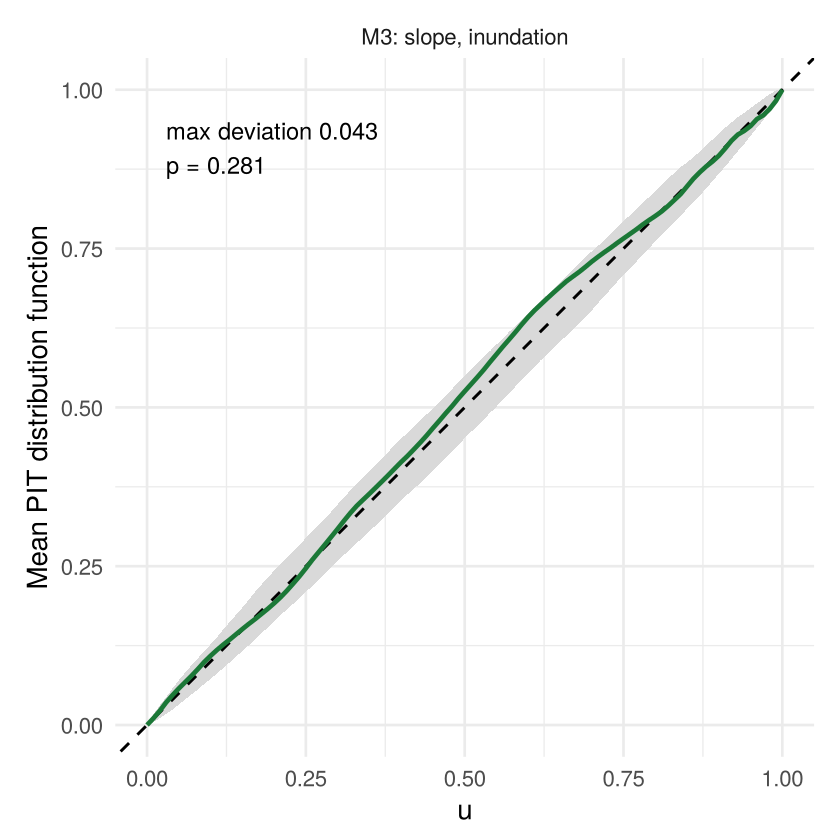
\includegraphics[width=0.45\textwidth]{cov_fit_pit.png}
\caption{Mean PIT distribution function of M3 among villages with positives (ten-fold cross-validation), with pointwise 95\% band from 1{,}000 simulated sets of counts.}
\label{fig:m3pit}
\end{figure}

\begin{figure}[H]
\centering
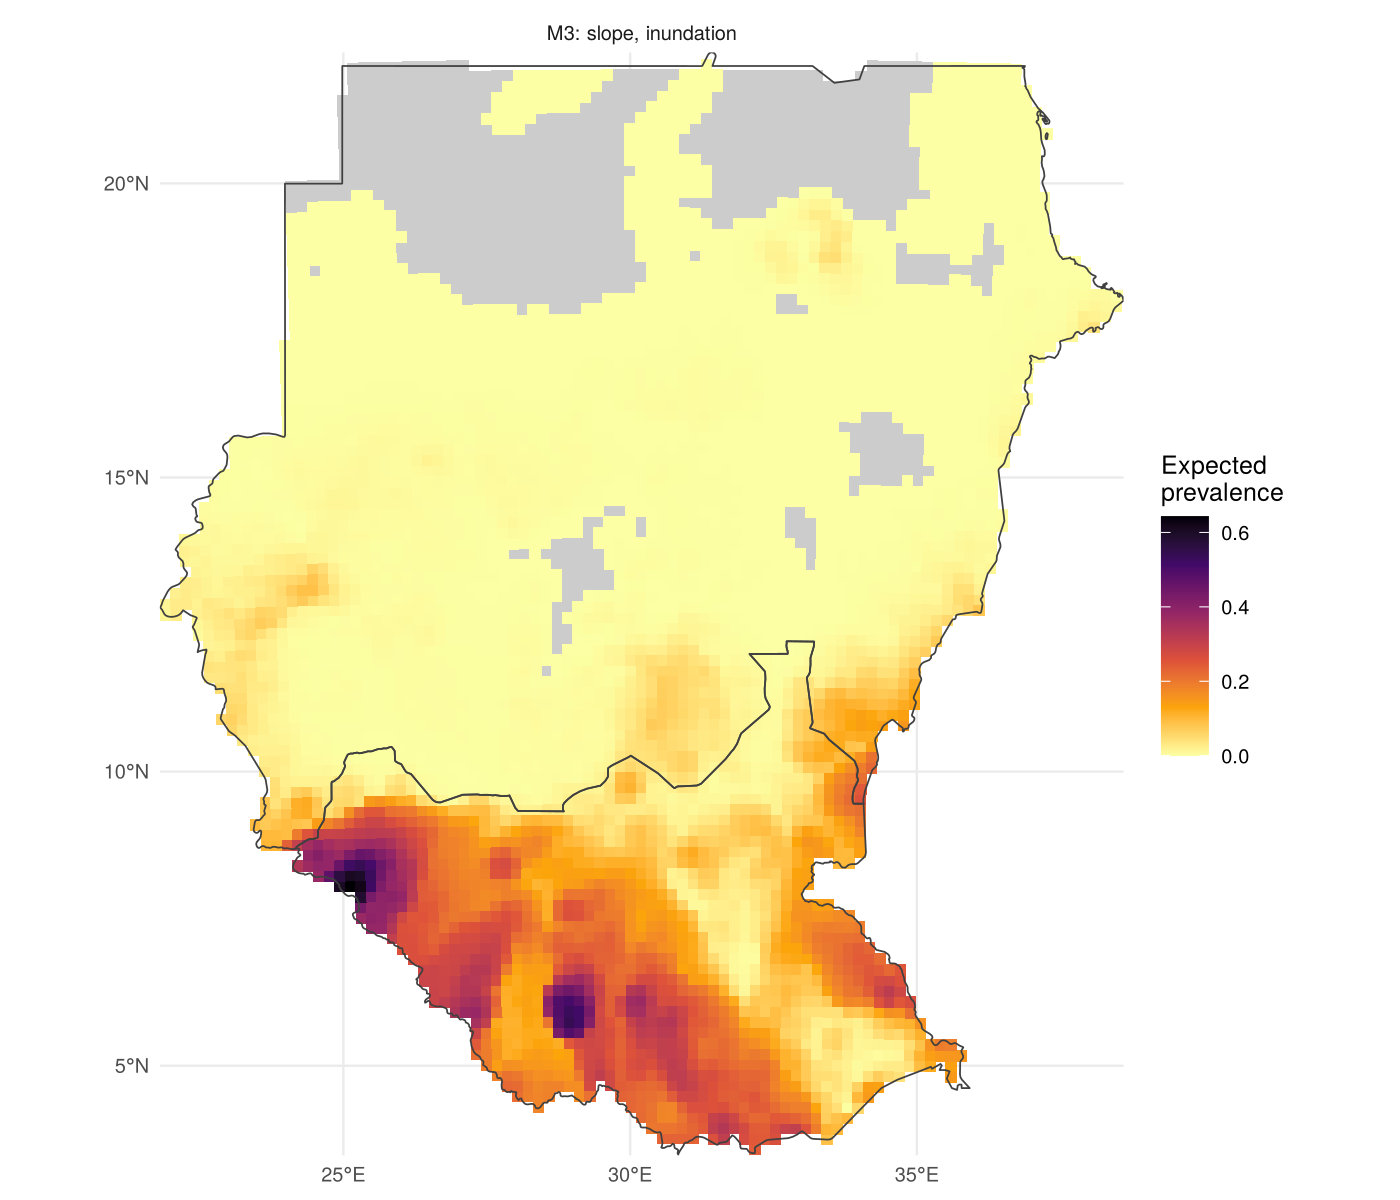
\includegraphics[width=0.7\textwidth]{cov_fit_prevalence_maps.png}
\caption{Expected prevalence of nodules from M3 on the 20~km grid (plug-in prediction at the estimates and the mode of $u$, village effect zero). Grey: beyond 40~km of every river, where the model predicts zero prevalence.}
\label{fig:m3map}
\end{figure}

\section{Comparison with Euclidean geostatistical models}\label{sec:gp}

To assess what the river network contributes, M3 was compared with two standard geostatistical models that use no river information. They keep the zero-inflated structure, aridity in both parts and the village effects, and replace $\log E$ by unit-variance Gaussian processes with exponential correlation $\exp(-2d/r)$ in straight-line distance $d$, with the parametrisation of the range used for the tail-down field:
\begin{align*}
\text{G1:}\quad & \mathrm{logit}\,\pi_i = a_0 + a_1 \log\AI_i + \alpha S(x_i), & \log\lambda_i &= b_0 + b_1 \log\AI_i + \gamma S(x_i) + Z_i,\\
\text{G2:}\quad & \mathrm{logit}\,\pi_i = a_0 + a_1 \log\AI_i + \alpha S_1(x_i), & \log\lambda_i &= b_0 + b_1 \log\AI_i + \gamma S_2(x_i) + Z_i,
\end{align*}
where in G1 one process $S$ enters both parts, with $\alpha > 0$ fixing its sign, and in G2 $S_1$ and $S_2$ are independent with a common range and $\alpha, \gamma > 0$. Each model has 8 parameters, against 11 for M3. They were fitted in the same way as M3: maximum likelihood with no priors, the Laplace approximation over the processes at the 900 villages and the village effects, the same treatment of multiple inner modes, and Wald intervals from the observed information. Cross-validation used the same ten folds; at a held-out village the processes are predicted by kriging from the training villages.

\begin{table}[H]
\centering
\small
\caption{Maximum likelihood estimates with 95\% Wald intervals of the Euclidean geostatistical models. Intervals for $\alpha$ (and $\gamma$ in G2), $r$ and $\sigma_Z$ are computed on the log scale.}
\label{tab:gpest}
\begin{tabular}{lcc}
\toprule
Parameter & G1: one process & G2: two processes \\
\midrule
$b_0$ (intercept, $\log\lambda$) & $-1.91$ ($-3.23$, $-0.59$) & $-1.49$ ($-2.24$, $-0.75$) \\
$b_1$ ($\log\AI$, $\log\lambda$) & 0.37 (0.02, 0.71) & 0.35 (0.05, 0.66) \\
$a_0$ (intercept, $\mathrm{logit}\,\pi$) & 1.18 ($-4.68$, 7.04) & 1.11 ($-1.18$, 3.40) \\
$a_1$ ($\log\AI$, $\mathrm{logit}\,\pi$) & 1.14 ($-0.34$, 2.62) & 1.22 (0.15, 2.28) \\
$\alpha$ (process in $\mathrm{logit}\,\pi$) & 4.56 (2.35, 8.85) & 3.67 (2.44, 5.50) \\
$\gamma$ (process in $\log\lambda$) & 1.02 (0.33, 1.72) & 0.67 (0.43, 1.05) \\
Range $r$ (km) & 1308 (341, 5018) & 760 (356, 1622) \\
$\sigma_Z$ & 0.48 (0.41, 0.56) & 0.47 (0.40, 0.55) \\
\bottomrule
\end{tabular}
\end{table}

\begin{table}[H]
\centering
\small
\caption{Comparison of M3 with the Euclidean models: approximate log-likelihood, number of parameters, AIC, and ten-fold cross-validation with the same random folds.}
\label{tab:gpcmp}
\footnotesize
\begin{tabular}{lccc}
\toprule
 & M3 (river network) & G1 & G2 \\
\midrule
Log-likelihood & $-1192.31$ & $-1186.32$ & $-1197.59$ \\
Parameters / AIC & 11 / 2406.6 & 8 / 2388.6 & 8 / 2411.2 \\
\midrule
Total logarithmic score & $-1155.0$ & $-1151.8$ & $-1155.4$ \\
\quad difference M3 $-$ model (block-bootstrap s.e.) & & $-3.2$ (6.4) & 0.4 (9.1) \\
Area under the ROC curve / Brier score & 0.953 / 0.082 & 0.956 / 0.079 & 0.955 / 0.081 \\
Expected villages without positives (550) & 546.5 & 539.6 & 556.4 \\
\quad of which sub-humid and humid (14) & 18.5 & 16.2 & 28.4 \\
Correlation of predicted and observed prevalence & 0.770 & 0.771 & 0.771 \\
Largest deviation of the mean PIT ($p$) & 0.043 (0.28) & 0.039 (0.35) & 0.058 (0.08) \\
\bottomrule
\end{tabular}
\end{table}

The shared process of G1 has a range of about 1{,}300~km, with a wide interval, and acts mainly as a smooth regional surface. Its ratio $\hat\alpha / \hat\gamma \approx 4.5$ is close to the ratio $\hat a_E / \hat\gamma \approx 5.3$ of the exposure in M3: in both models one spatial component drives the probability and the intensity of transmission in nearly fixed proportion. G2, which makes the two parts independent, has a log-likelihood 11 units lower than G1 with the same number of parameters, and overestimates the number of humid villages without positives (28.4 against 14 observed).

G1 has the highest log-likelihood and the best cross-validated scores (Table~\ref{tab:gpcmp}). The differences in prediction from M3 are small, however. The total logarithmic score of M3 is 3.2 units lower than that of G1, about 0.004 per village, with a standard error of 6.4 from a bootstrap of $1^\circ$ cells (95\% interval $-15.3$ to 10.1), and M3 has the better score at 53\% of the villages. It is 0.4 units higher than that of G2 (standard error 9.1). The AUC and Brier scores differ in the third decimal place, all three models are calibrated among villages with positives (Figure~\ref{fig:gppit}), and the prevalence maps on the grid are correlated 0.96 (Figure~\ref{fig:gpmaps}). The difference in log-likelihood, 6.0 units in favour of G1 with three fewer parameters, should be read with caution: the Laplace approximation integrates over at most 2{,}700 random effects in the Euclidean models and over 145{,}329 graph values and 900 village effects in M3, and its error need not be the same in the two cases.

\begin{figure}[H]
\centering
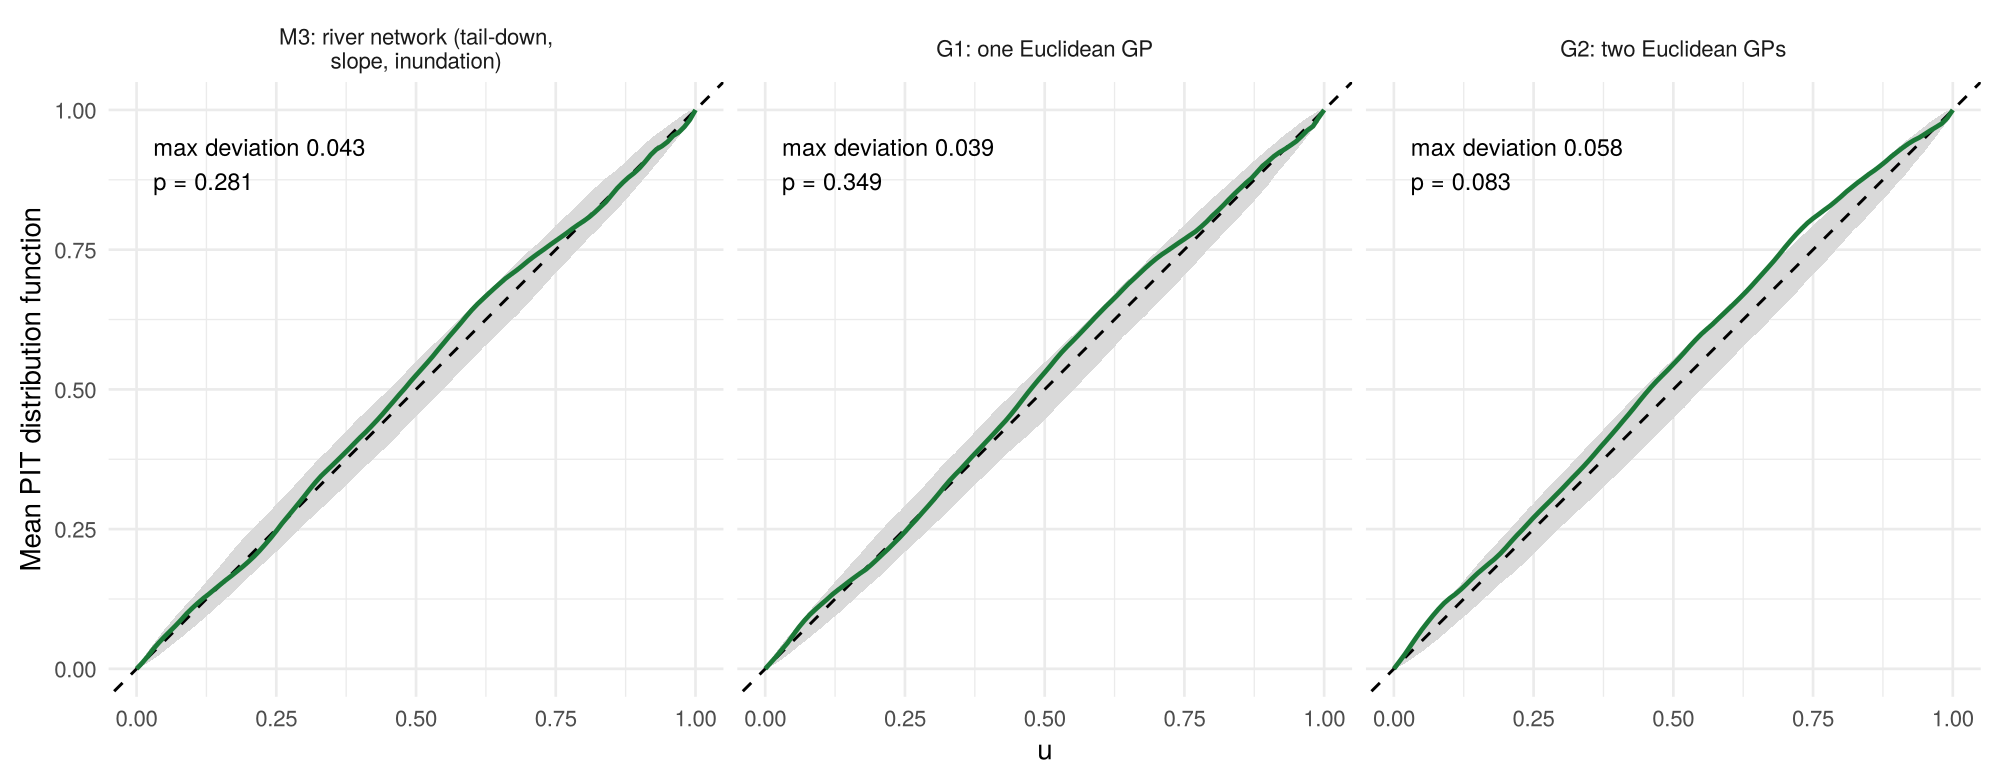
\includegraphics[width=\textwidth]{m3_vs_gp_pit.png}
\caption{Mean PIT distribution functions among villages with positives (ten-fold cross-validation, same folds) of M3 and the Euclidean models G1 and G2, with pointwise 95\% bands.}
\label{fig:gppit}
\end{figure}

\begin{figure}[H]
\centering
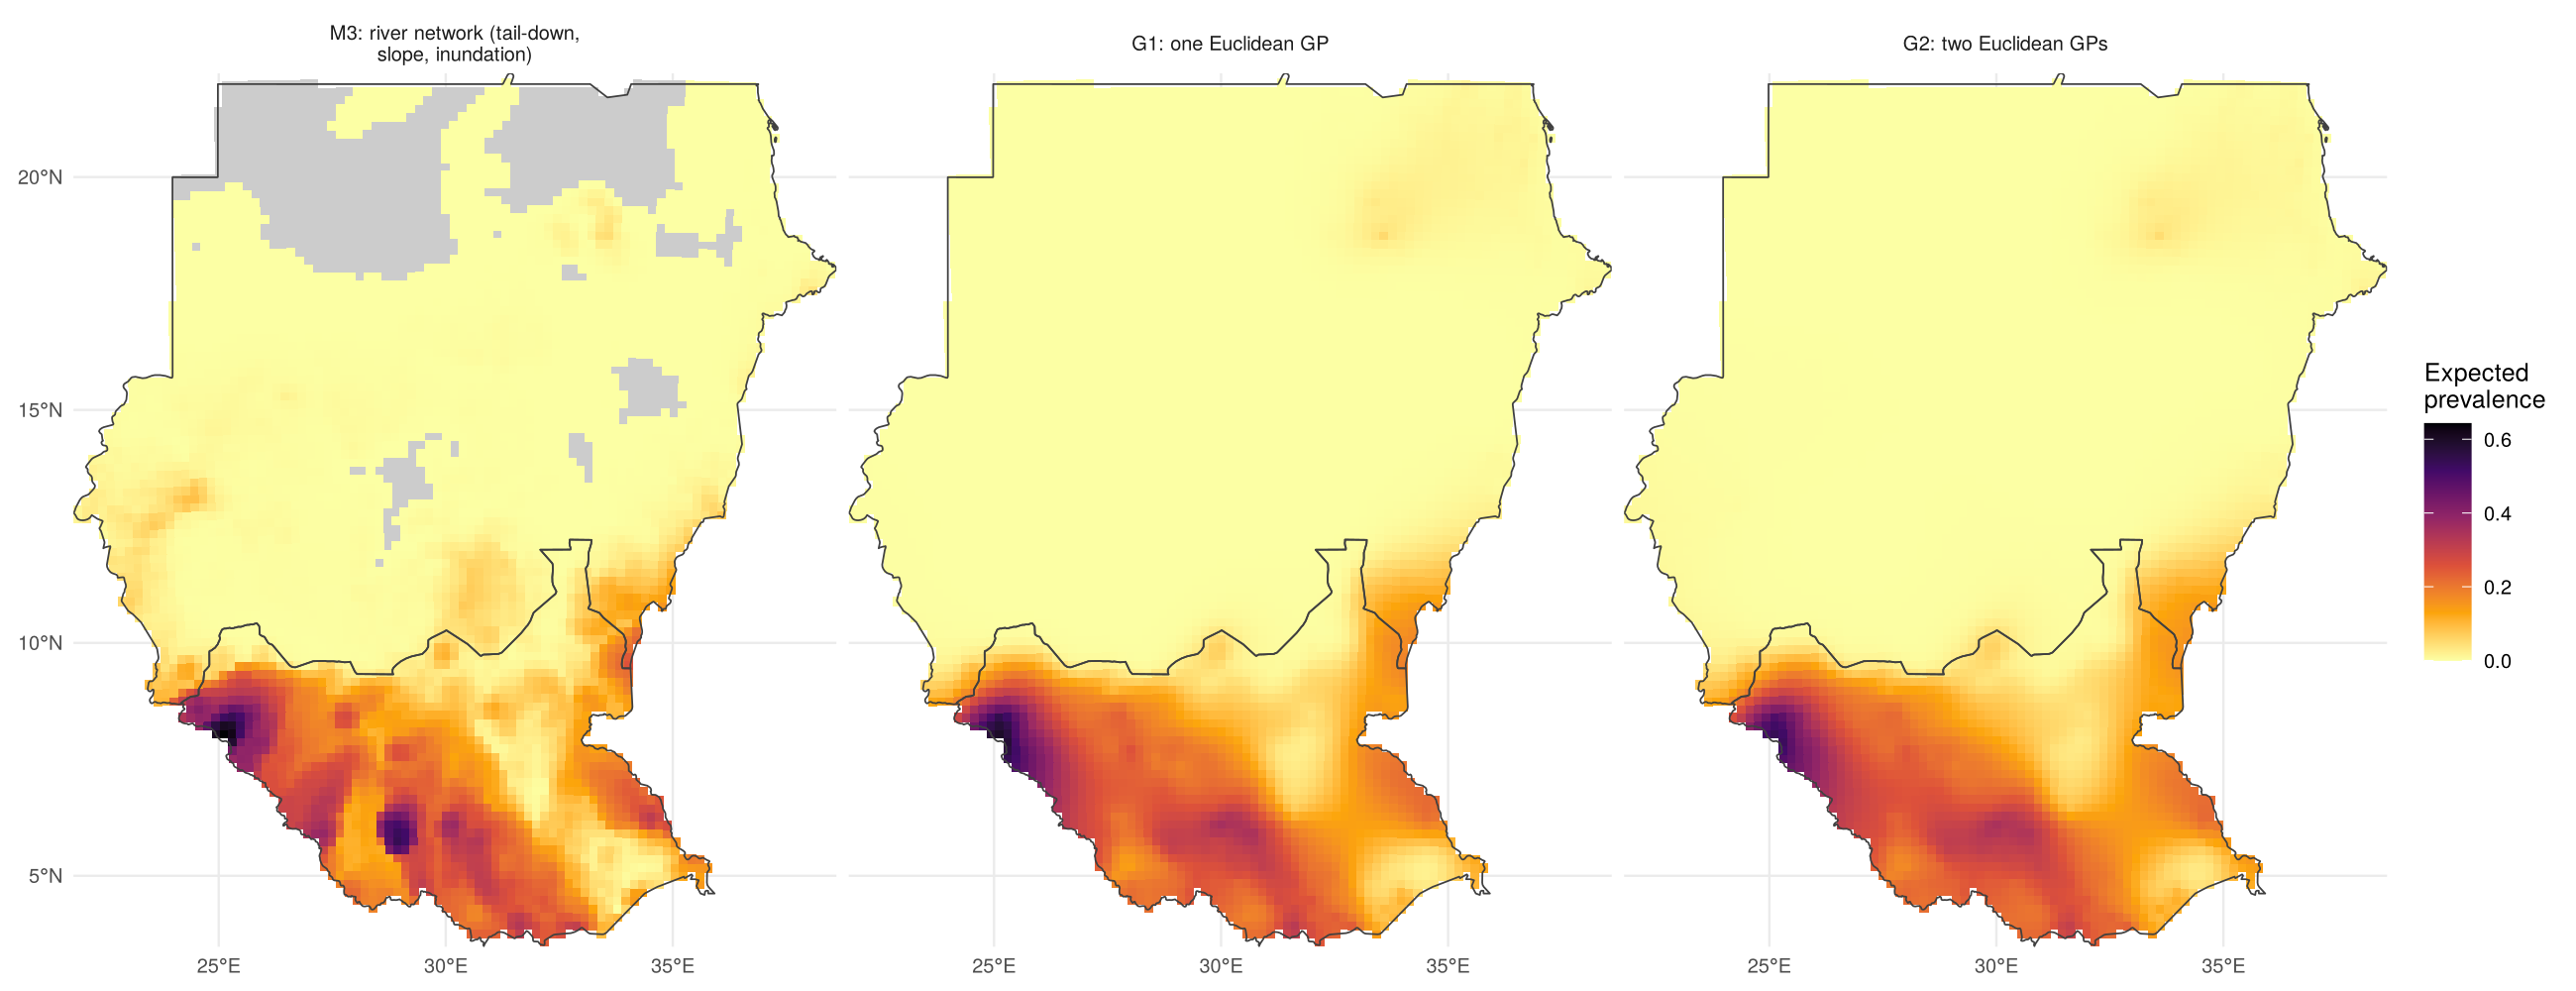
\includegraphics[width=\textwidth]{m3_vs_gp_prevalence_maps.png}
\caption{Expected prevalence on the 20~km grid from M3 (grey: zero exposure) and from the Euclidean models G1 and G2.}
\label{fig:gpmaps}
\end{figure}

The two kinds of model therefore interpolate the surveyed villages about equally well, and random folds favour the Euclidean models by construction: a held-out village almost always has surveyed neighbours, which a smooth long-range surface uses directly. The river-network model reaches a similar predictive accuracy while offering what a Euclidean process cannot. It predicts zero transmission where there are no rivers within reach, whereas G1 and G2 can only predict low prevalence, which reverts to the mean away from the data (in the cells with zero exposure in M3 their predicted prevalence is up to 2.5\%). Its prediction has a mechanism: risk comes from breeding on particular reaches, and the habitat covariates act with the directions expected from the biology of the vector. In unsurveyed areas its predictions follow the river network and the habitat along it, so that it can identify a potential focus on a steep river far from the surveys, whereas the Euclidean predictions follow only the distance to surveyed villages. It indicates which reaches and basins drive transmission, the information needed to target larviciding or the search for breeding sites. And its dependence follows the connectivity of the rivers rather than straight lines across watersheds.


\appendix
\section{Exploratory figures for individual covariates}

Each figure shows (a) the village average of the covariate within 40~km, (b) the share of villages with at least one positive and (c) prevalence among villages with positives by quintile of the village average, with 95\% Wilson intervals (black) and within terciles of aridity (thin lines), and (d)--(e) the Spearman correlations of the two parts against the kernel range, pooled with a 95\% spatial block-bootstrap band and within the middle and humid terciles; the dashed line marks 40~km.

\begin{figure}[H]\centering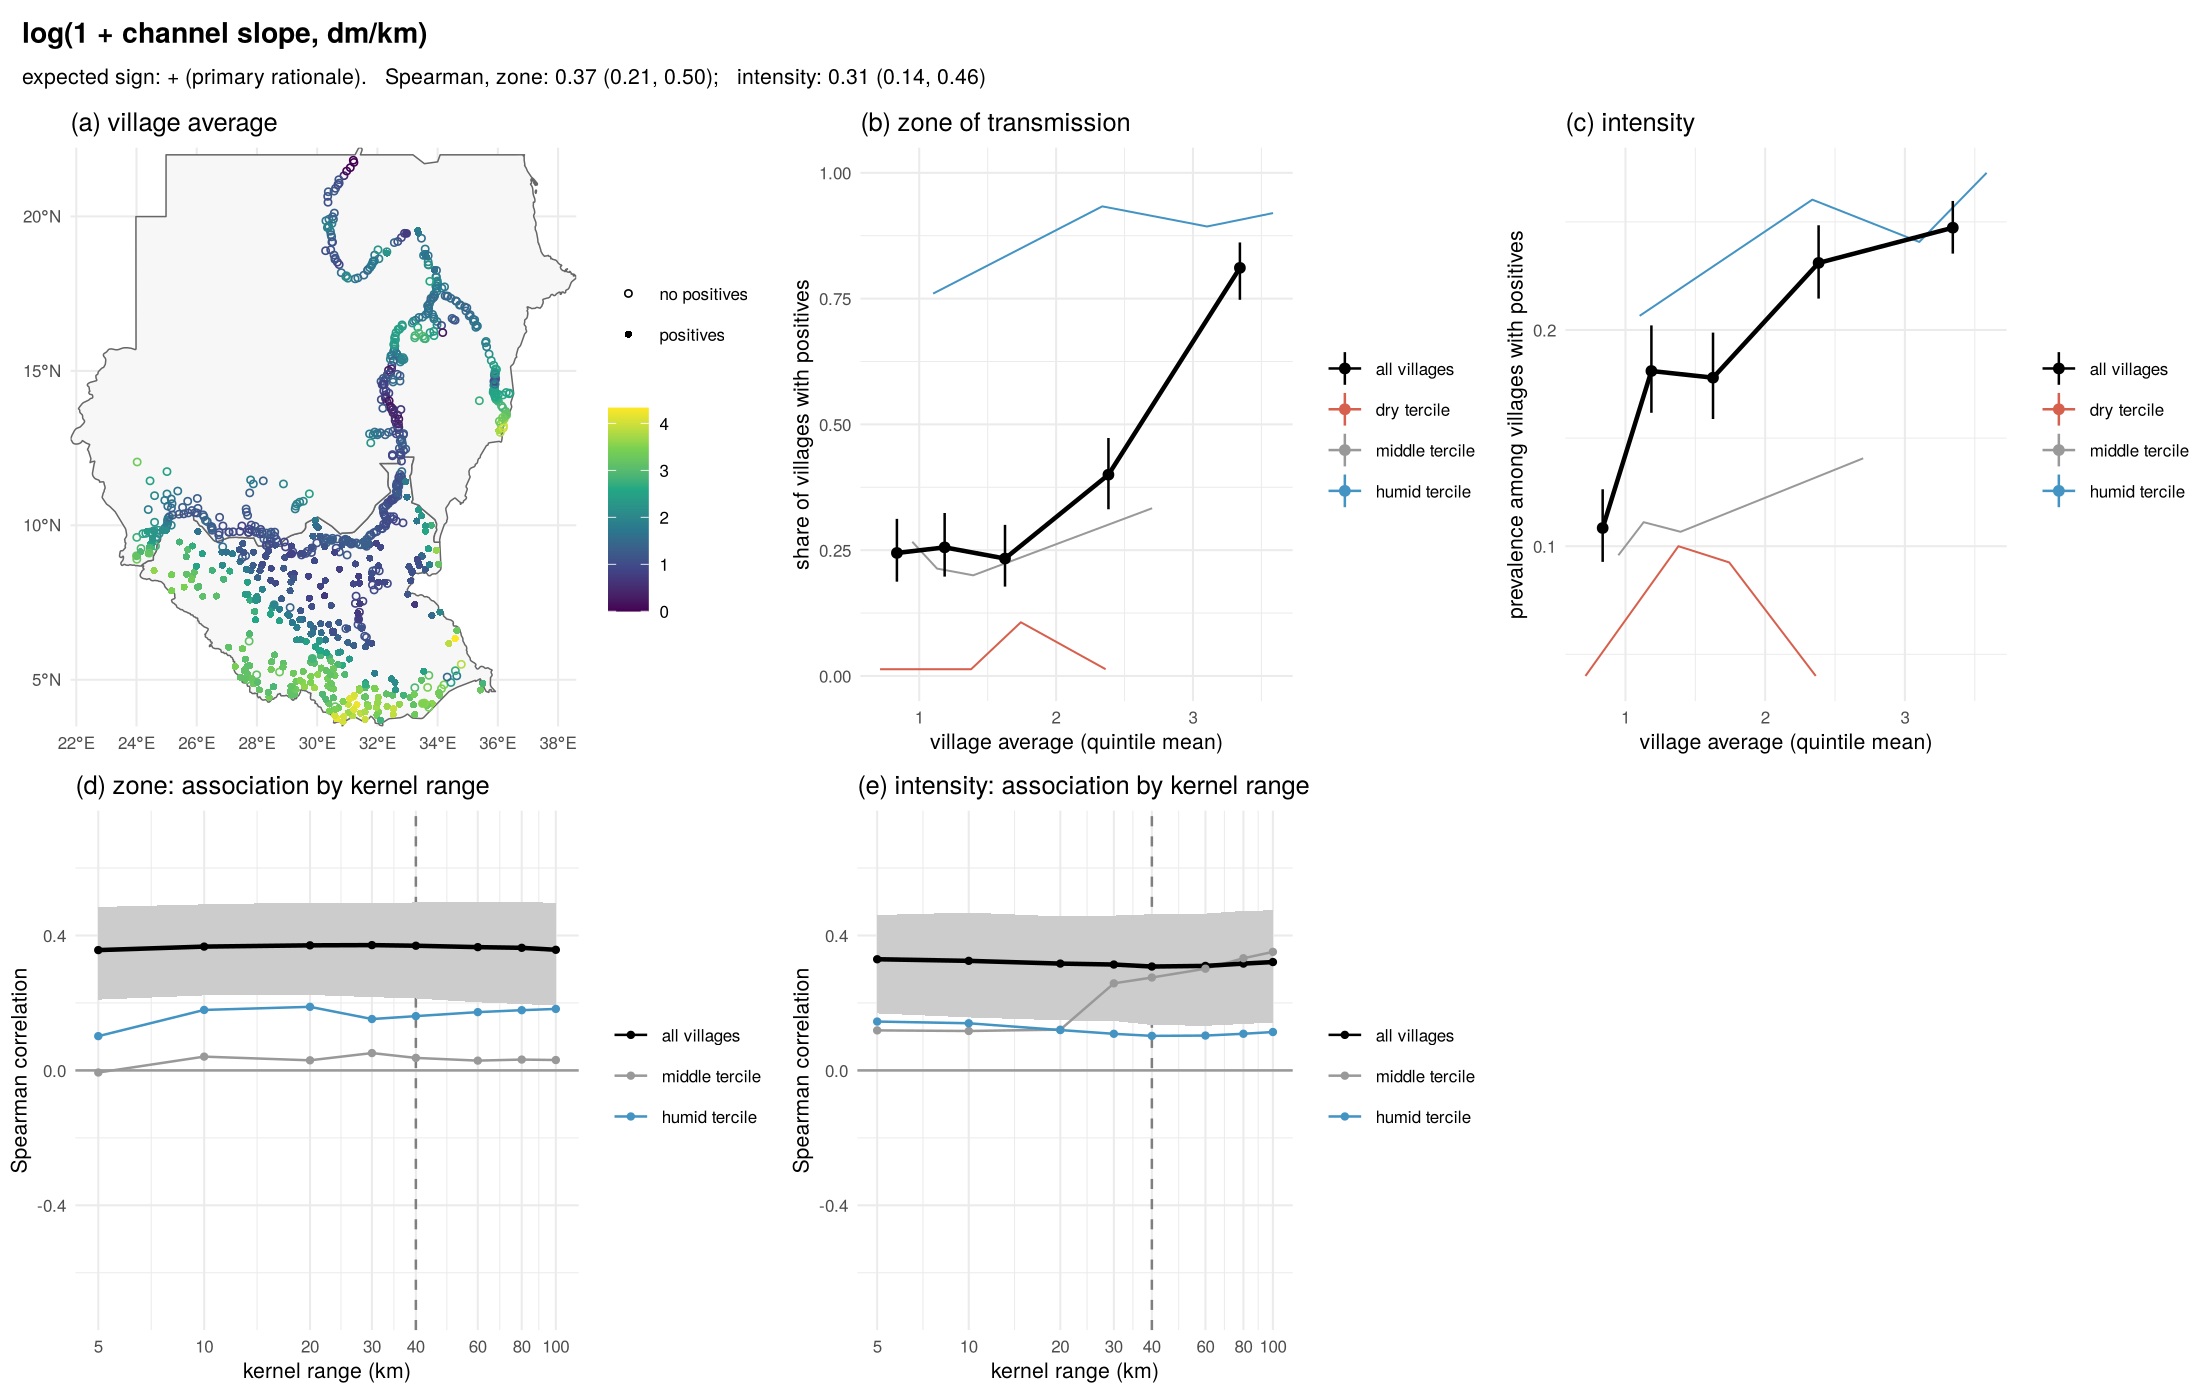
\includegraphics[width=\textwidth]{eda_log_slope.png}\caption{Channel slope.}\end{figure}
\begin{figure}[H]\centering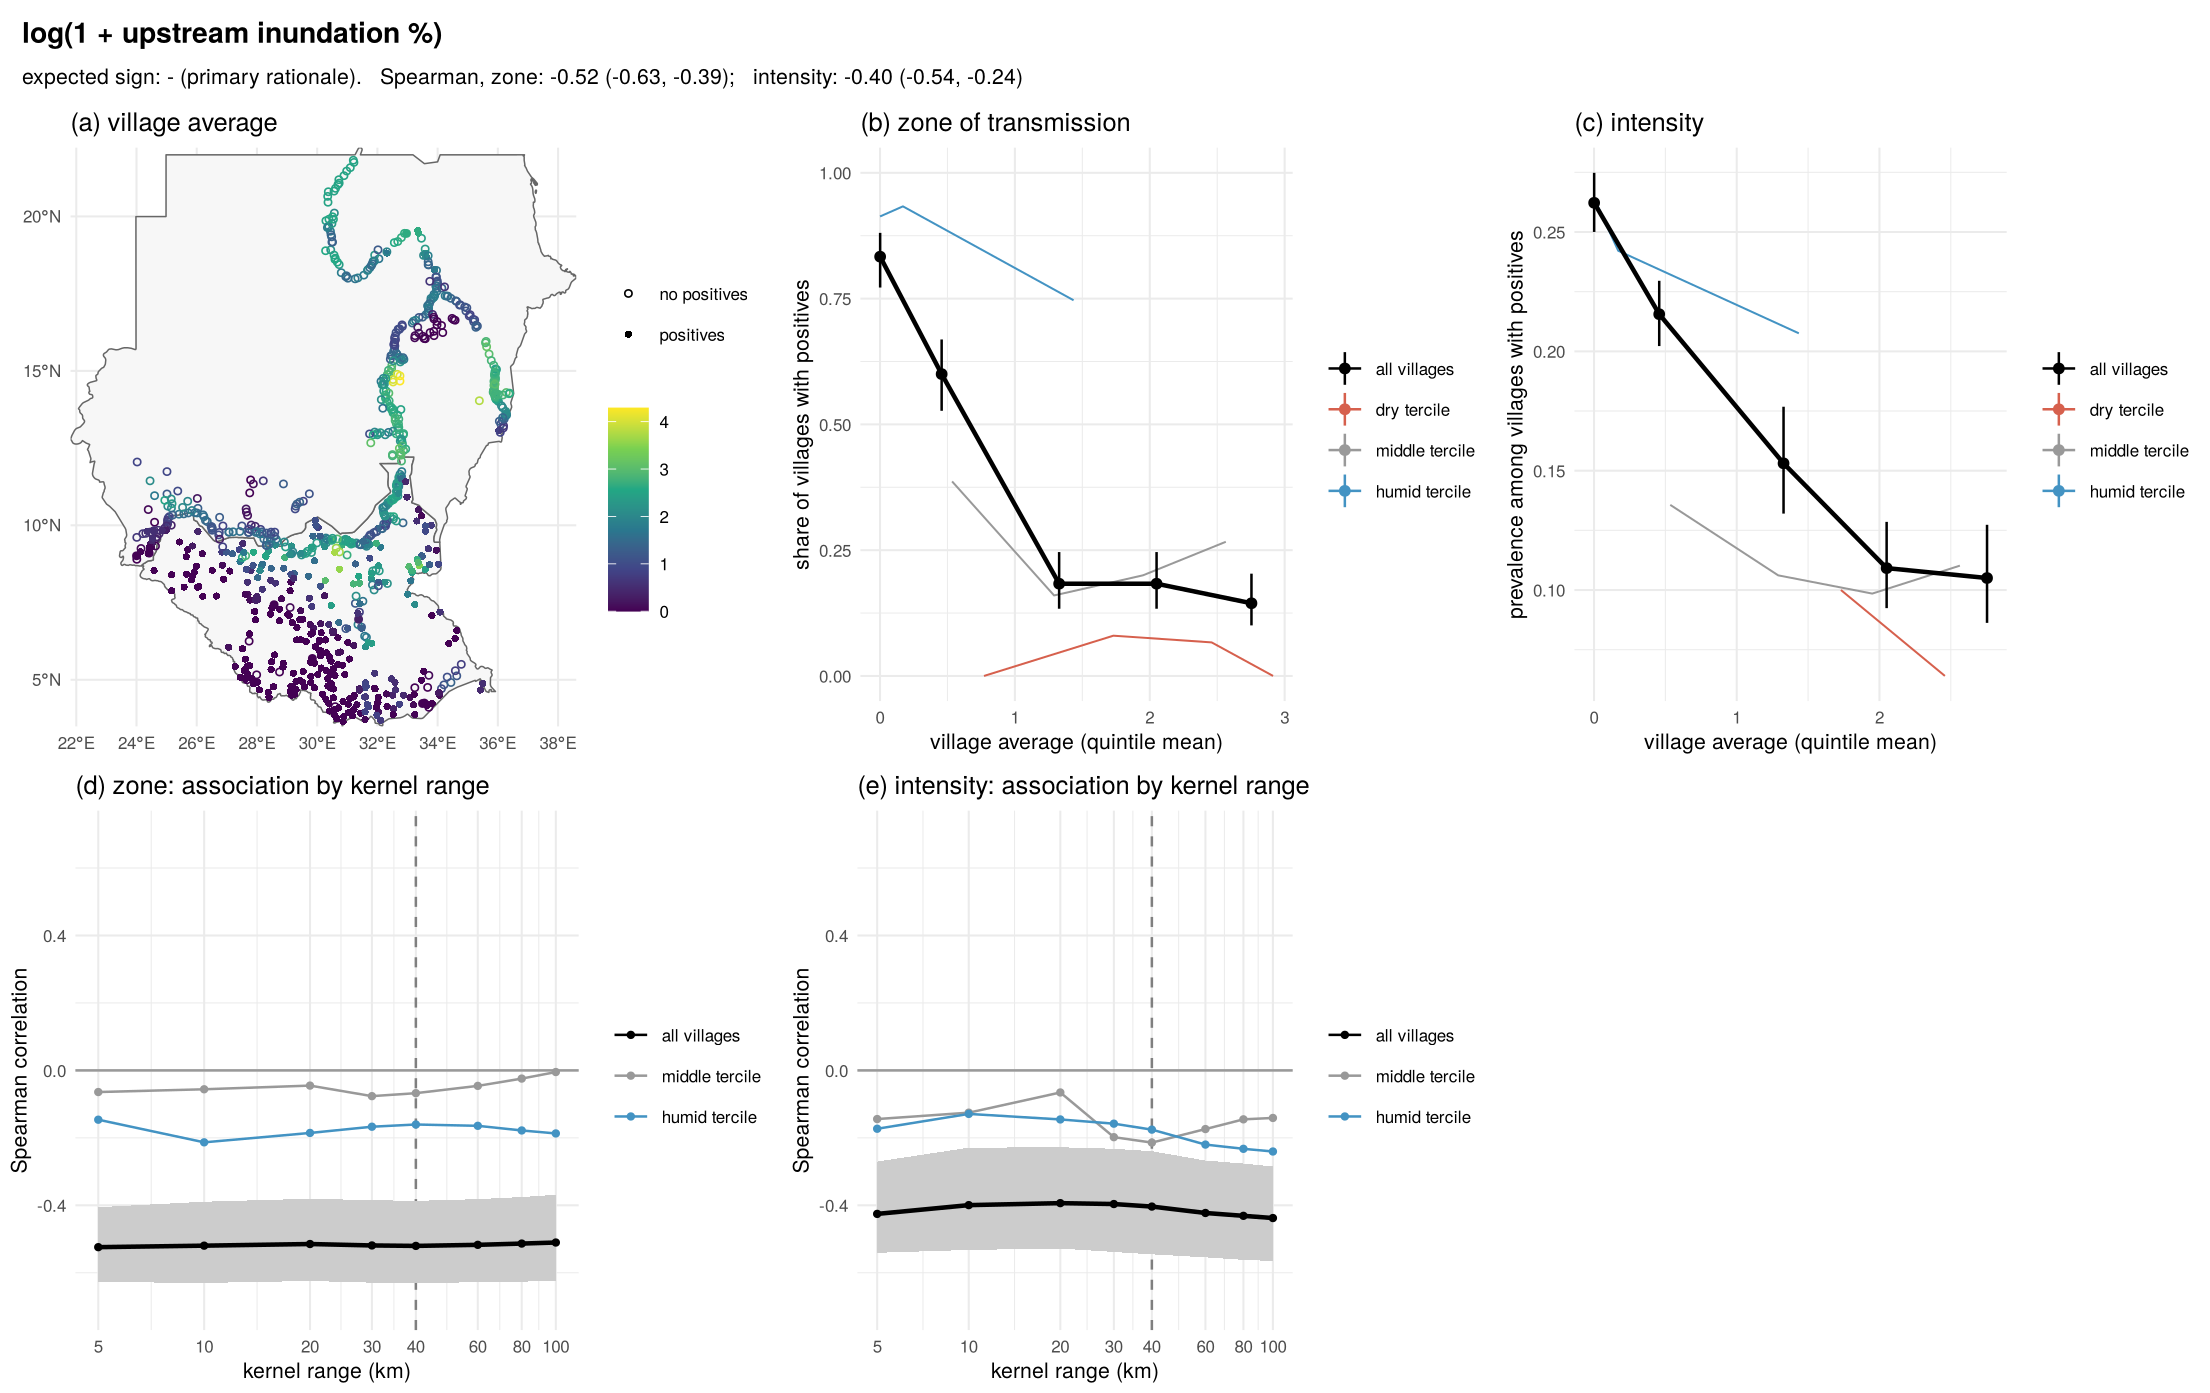
\includegraphics[width=\textwidth]{eda_inundation.png}\caption{Upstream inundation.}\end{figure}
\begin{figure}[H]\centering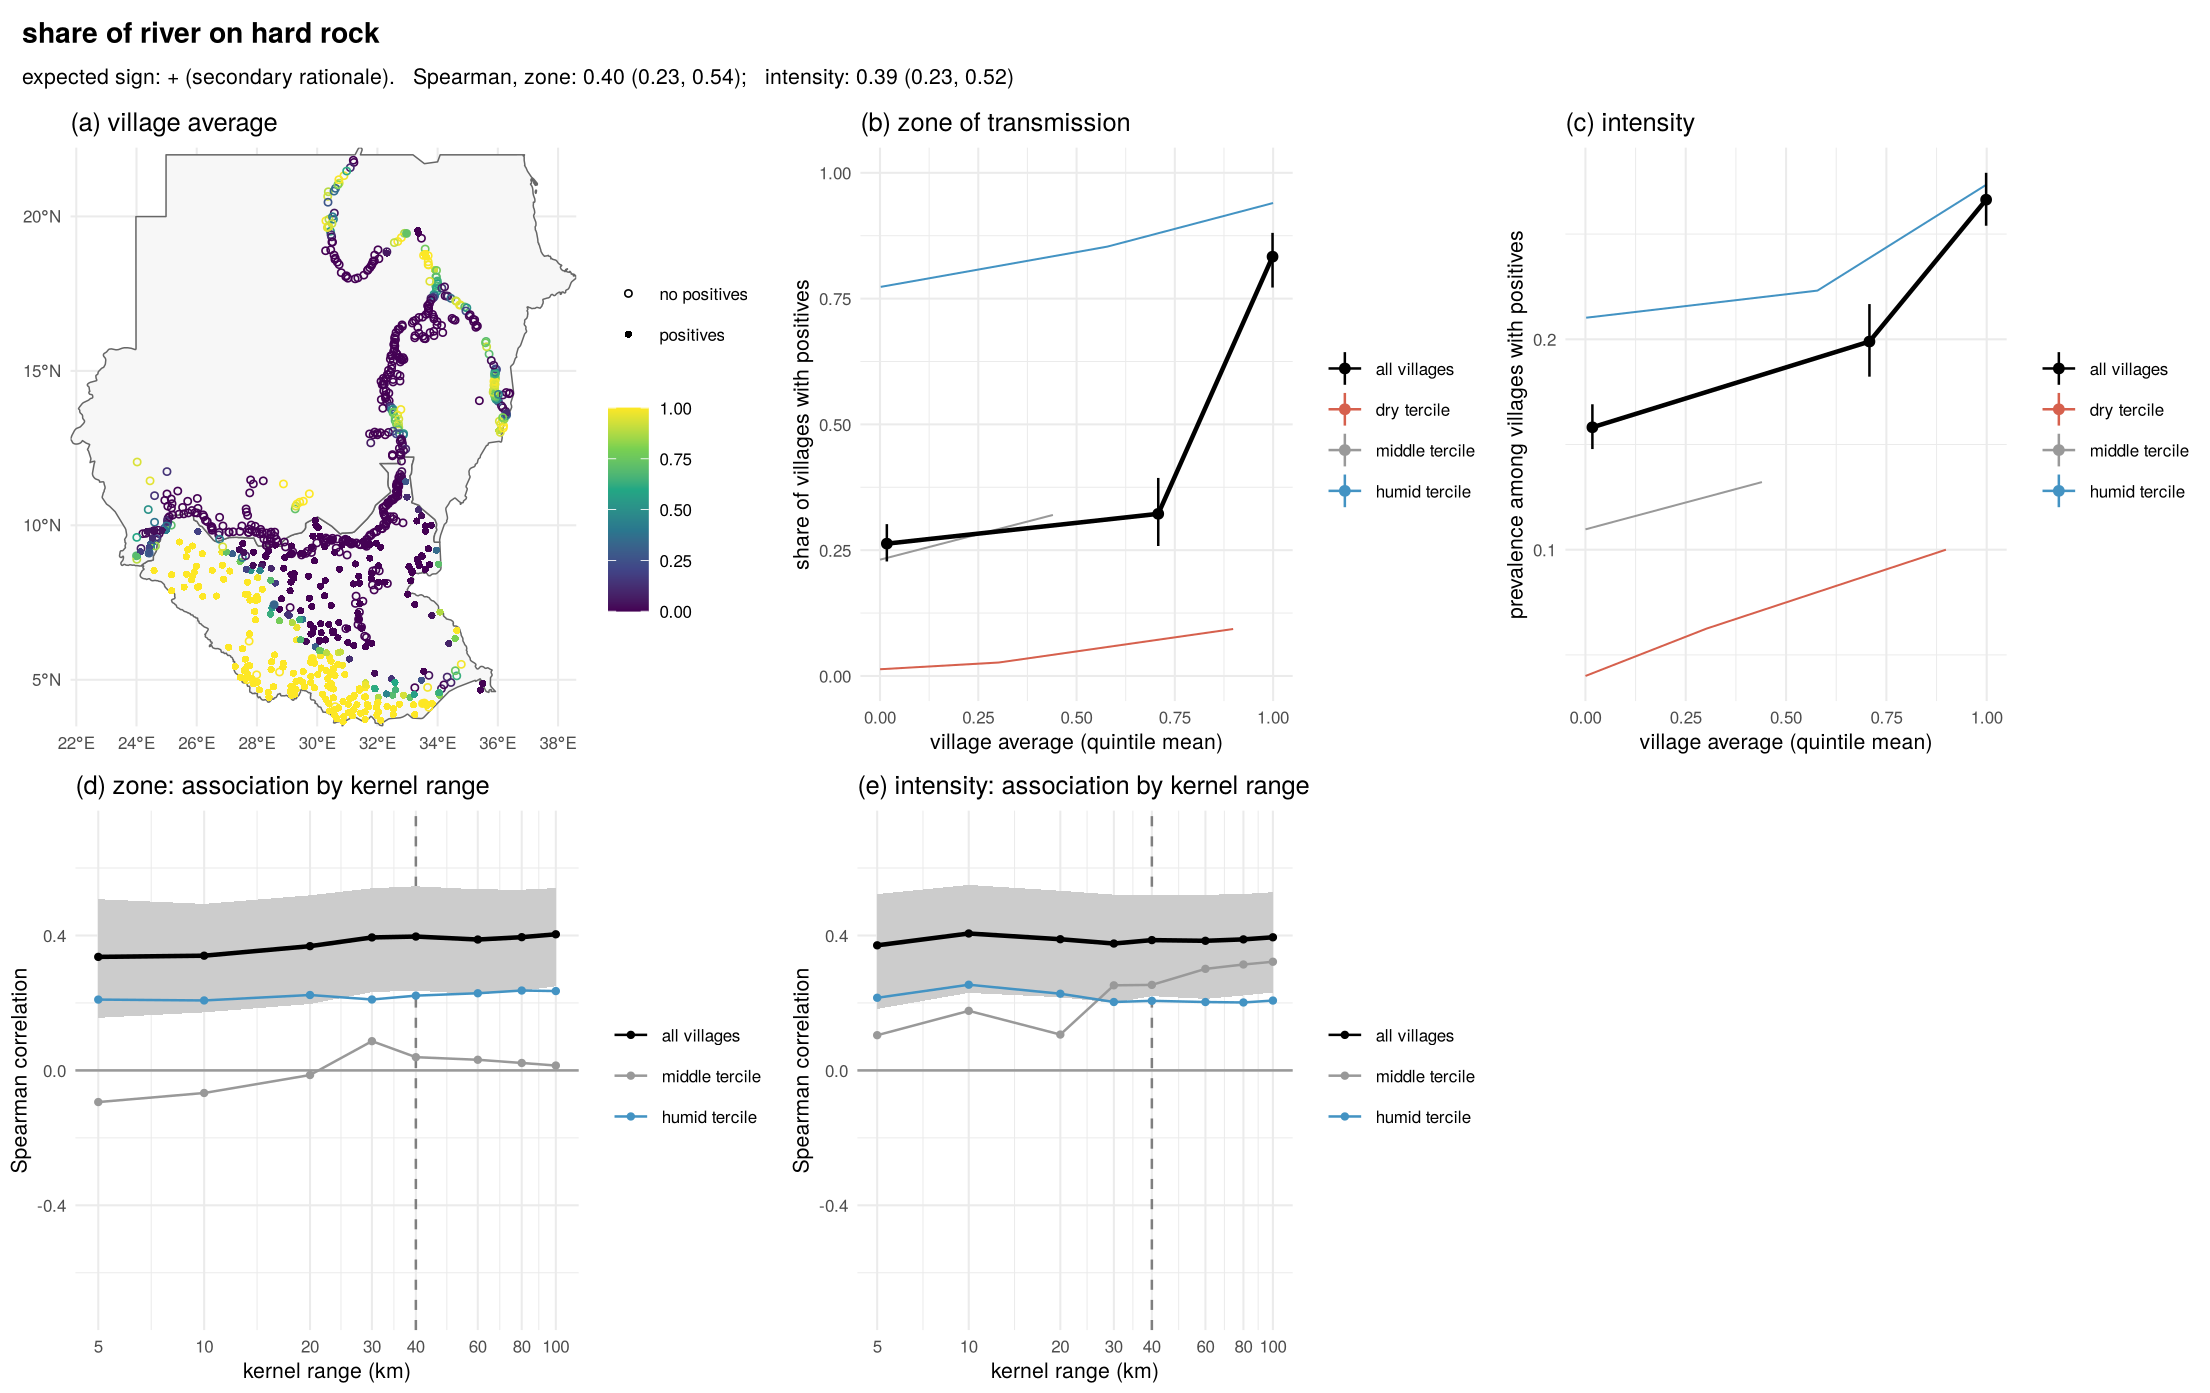
\includegraphics[width=\textwidth]{eda_hard_rock.png}\caption{Hard rock.}\end{figure}
\begin{figure}[H]\centering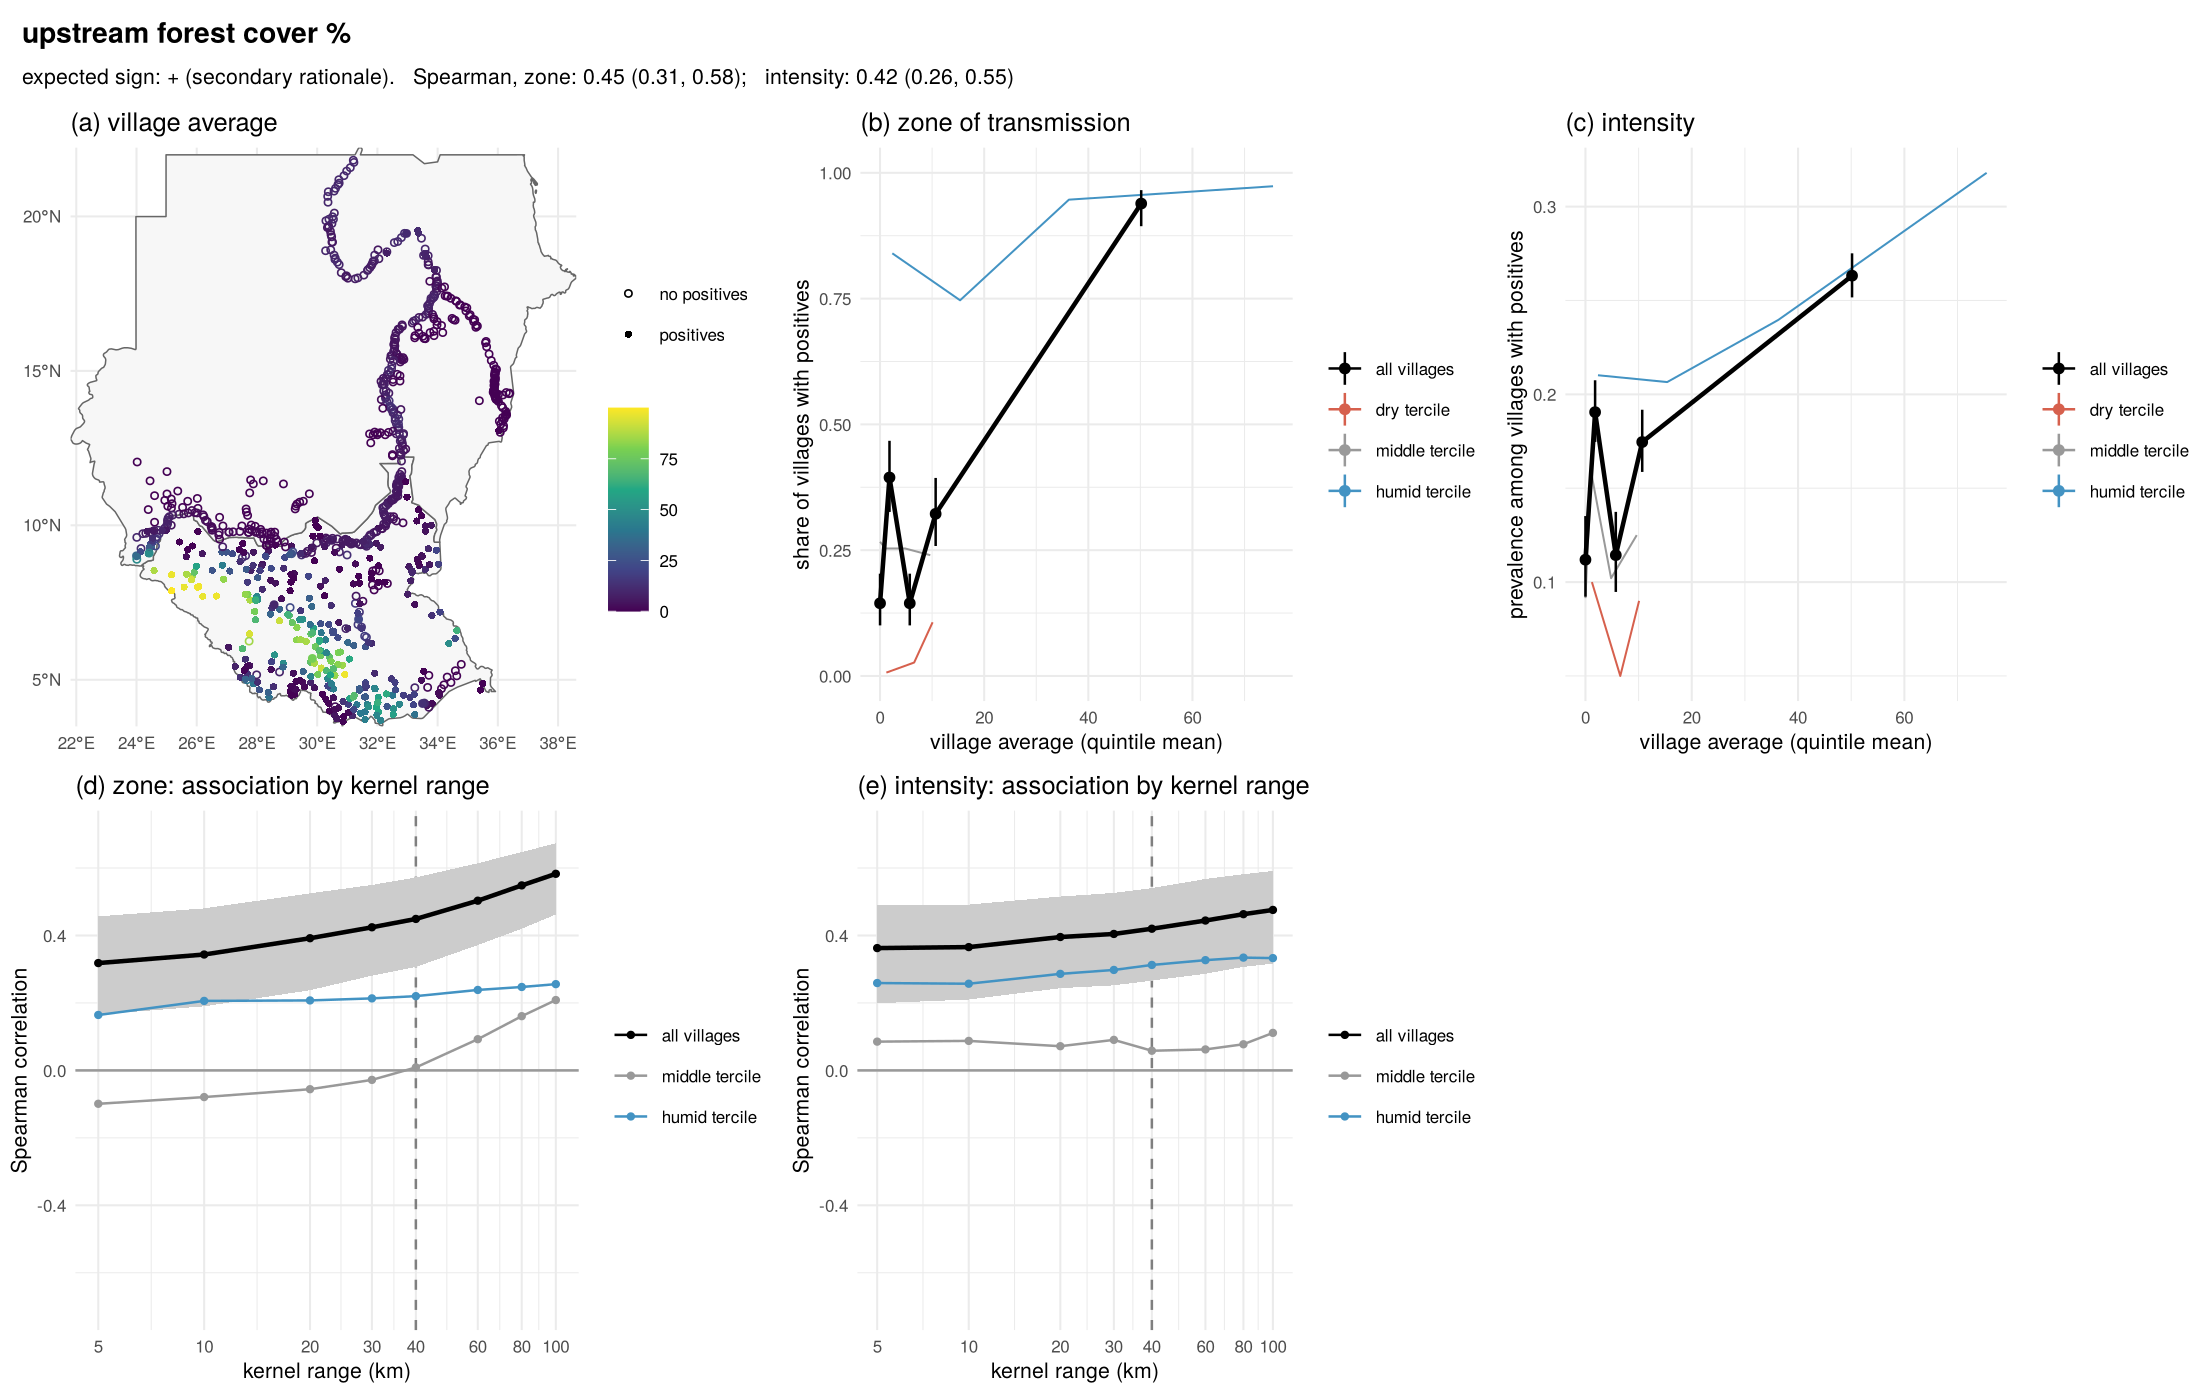
\includegraphics[width=\textwidth]{eda_forest.png}\caption{Upstream forest cover (not selected).}\end{figure}
\begin{figure}[H]\centering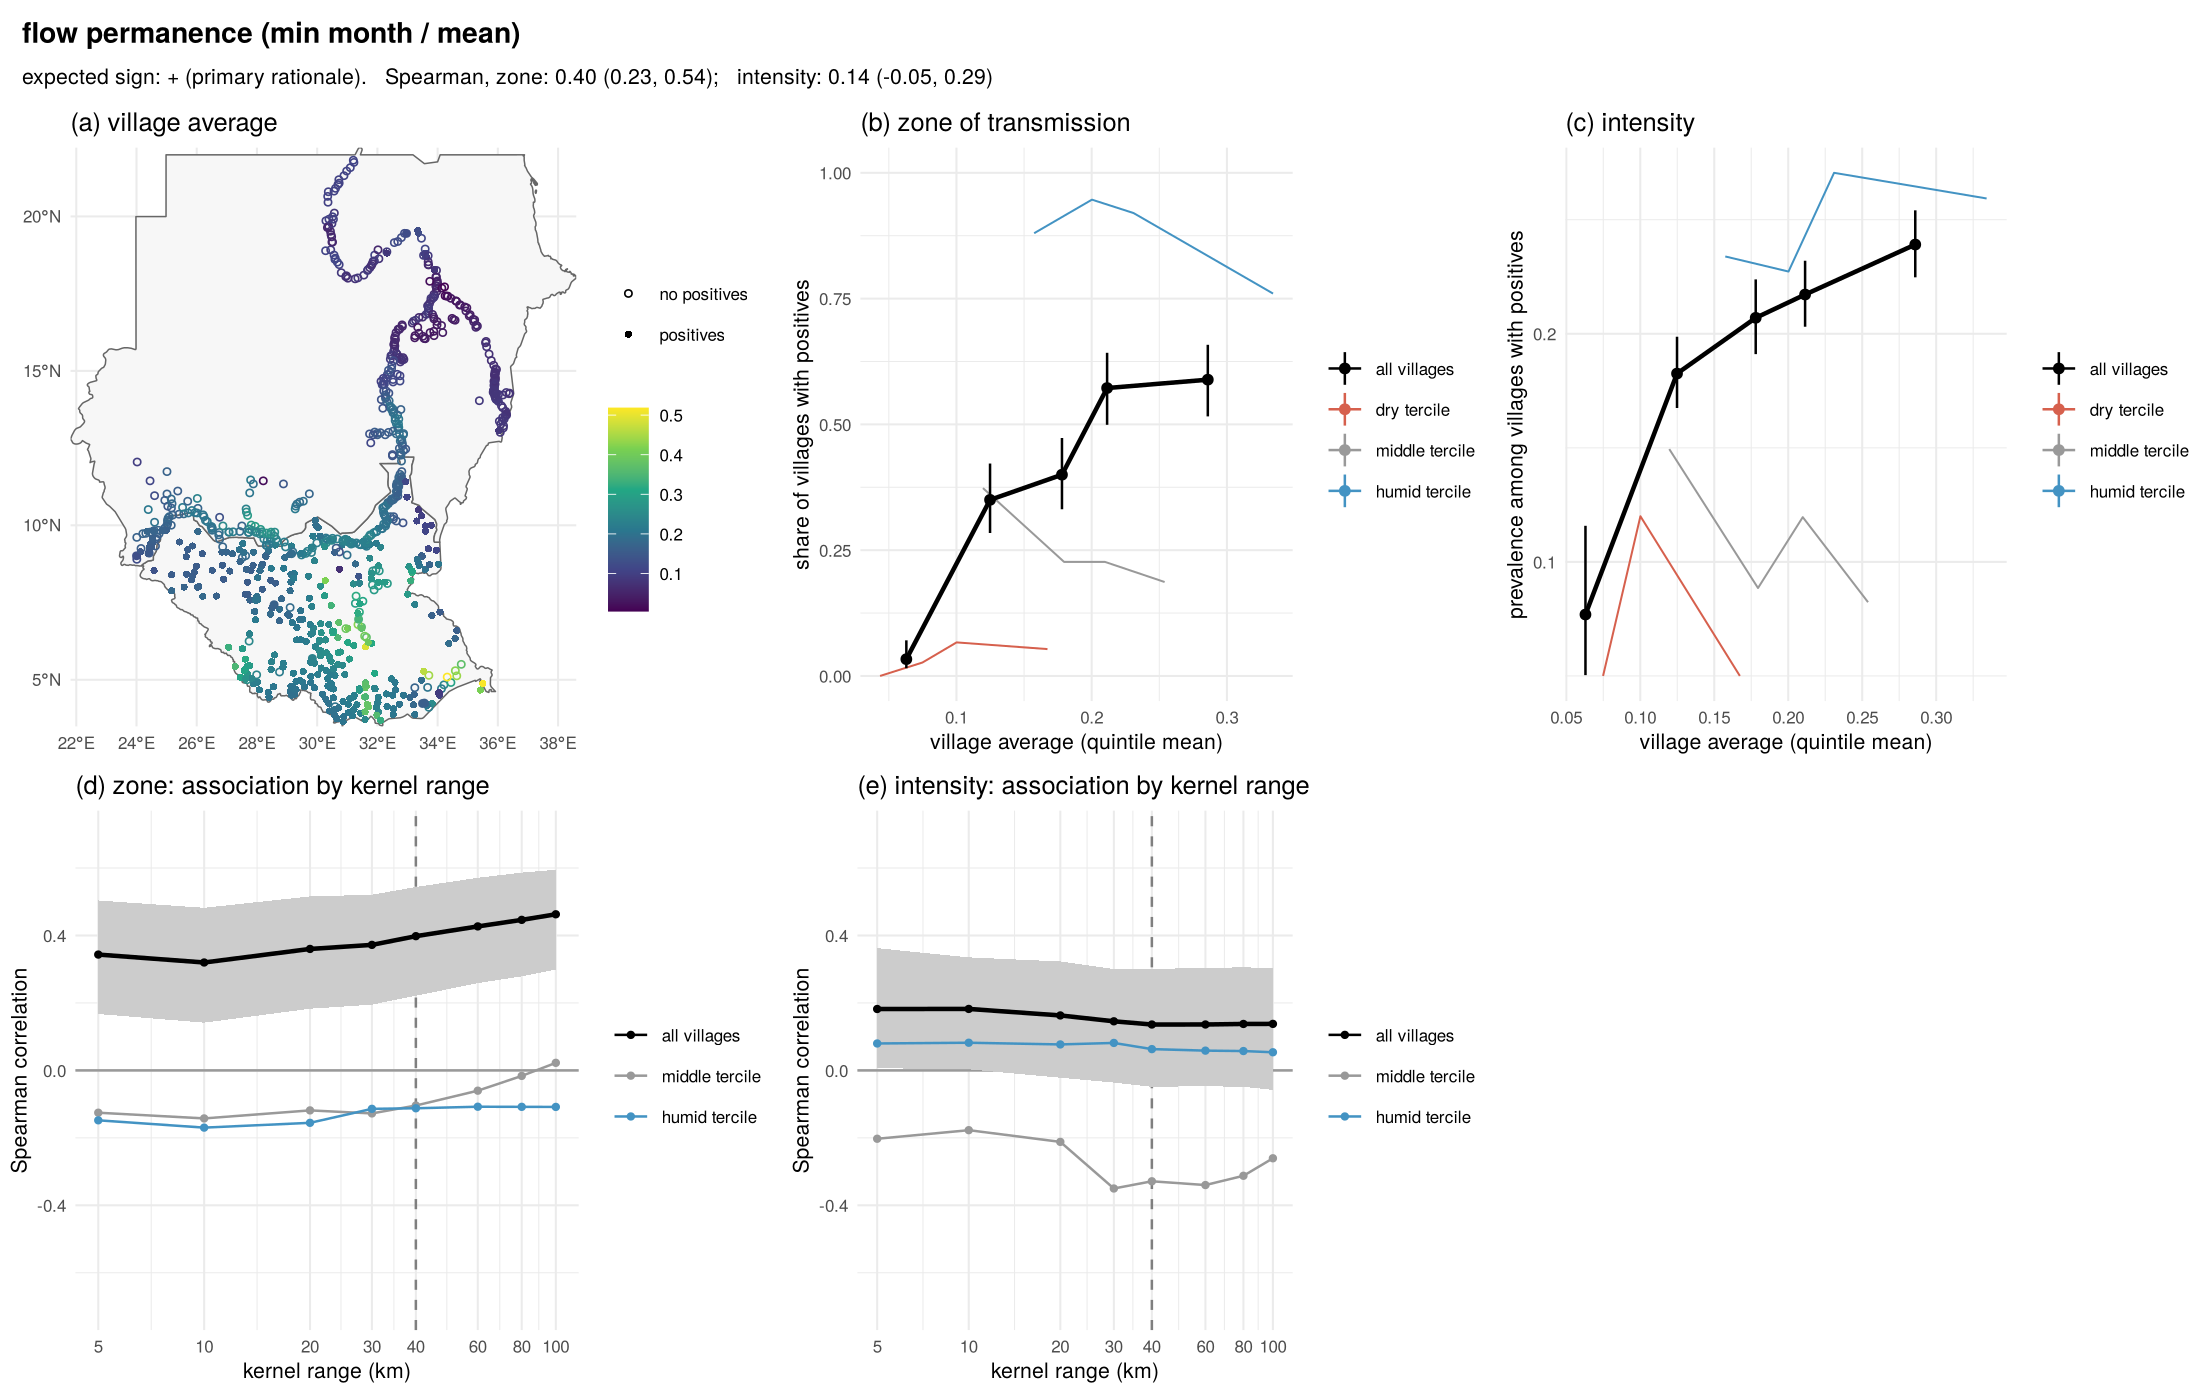
\includegraphics[width=\textwidth]{eda_permanence.png}\caption{Flow permanence (not selected).}\end{figure}

\begin{thebibliography}{99}
\bibitem[Bolin et al.(2024)]{bolin2024} Bolin, D., Simas, A.~B. and Wallin, J. (2024). Gaussian Whittle--Mat\'ern fields on metric graphs. \textit{Bernoulli}, 30(2), 1611--1639.
\bibitem[Bolin et al.(2026)]{bolin2026dir} Bolin, D., Simas, A.~B., Karlsson Strandh, E. and Wallin, J. (2026). Gaussian processes on directed metric graphs. arXiv:2609.01435.
\bibitem[Carnaghi et al.(2024)]{carnaghi2024} Carnaghi, M. et al. (2024). Short- and long-range dispersal by members of the \textit{Simulium damnosum} complex (Diptera: Simuliidae), vectors of onchocerciasis: a review. \textit{Insects}, 15(8), 606.
\bibitem[Crosskey(1990)]{crosskey1990} Crosskey, R.~W. (1990). \textit{The Natural History of Blackflies}. Chichester: Wiley.
\bibitem[Czado et al.(2009)]{czado2009} Czado, C., Gneiting, T. and Held, L. (2009). Predictive model assessment for count data. \textit{Biometrics}, 65, 1254--1261.
\bibitem[Hartmann and Moosdorf(2012)]{hartmann2012} Hartmann, J. and Moosdorf, N. (2012). The new global lithological map database GLiM: a representation of rock properties at the Earth surface. \textit{Geochemistry, Geophysics, Geosystems}, 13, Q12004.
\bibitem[Lehner and Grill(2013)]{lehner2013} Lehner, B. and Grill, G. (2013). Global river hydrography and network routing: baseline data and new approaches to study the world's large river systems. \textit{Hydrological Processes}, 27, 2171--2186.
\bibitem[Linke et al.(2019)]{linke2019} Linke, S., Lehner, B., Ouellet Dallaire, C., Ariwi, J., Grill, G., Anand, M., Beames, P., Burchard-Levine, V., Maxwell, S., Moidu, H., Tan, F. and Thieme, M. (2019). Global hydro-environmental sub-basin and river reach characteristics at high spatial resolution. \textit{Scientific Data}, 6, 283.
\bibitem[Steihaug(1983)]{steihaug1983} Steihaug, T. (1983). The conjugate gradient method and trust regions in large scale optimization. \textit{SIAM Journal on Numerical Analysis}, 20(3), 626--637.
\bibitem[Ver Hoef and Peterson(2010)]{verhoef2010} Ver Hoef, J.~M. and Peterson, E.~E. (2010). A moving average approach for spatial statistical models of stream networks. \textit{Journal of the American Statistical Association}, 105(489), 6--18.
\bibitem[Wendland(1995)]{wendland1995} Wendland, H. (1995). Piecewise polynomial, positive definite and compactly supported radial functions of minimal degree. \textit{Advances in Computational Mathematics}, 4, 389--396.
\bibitem[Zomer et al.(2022)]{zomer2022} Zomer, R.~J., Xu, J. and Trabucco, A. (2022). Version 3 of the Global Aridity Index and Potential Evapotranspiration Database. \textit{Scientific Data}, 9, 409.
\end{thebibliography}

\end{document}
